\documentclass[UTF8]{ctexart}

\usepackage{subfiles}  

%下面的语句, 引入你的头部设置文件
\usepackage{C:/phpStorm_proj/02_myself_ID_EGO/+100_latex_all_math_sel/myPreamble} 
%必须是绝对路径,才能让各个tex在单独编译时使用到

\title{行列式}


%---------------------------------


\begin{document}
	\tableofcontents % 生成目录
	\date{} % 若不写这句, 则默认也会渲染出日期, 所以我们要手动赋空值
	\maketitle  %这行代码, 让你前面的 title, author, date生效
	
	
	
	
	\section{二阶与三阶行列式}
	
	\subsection{二阶行列式}
	
	$
	\left| \begin{matrix}
		a&		b\\
		c&		d\\
	\end{matrix} \right|=\underset{\text{主对角线}}{\underbrace{ad}}-\underset{\text{副对角线}}{\underbrace{bc}}
	$
	

~\\
\hrule
~\\

	
		\subsection{三阶行列式}
	$
	\left| \begin{matrix}
		a&		b&		c\\
		d&		e&		f\\
		h&		i&		j\\
	\end{matrix} \right|=\left( aej+bfh+cdi \right) -\left( ceh+dbj+aif \right) 
	$ \\
	
	即: \\
	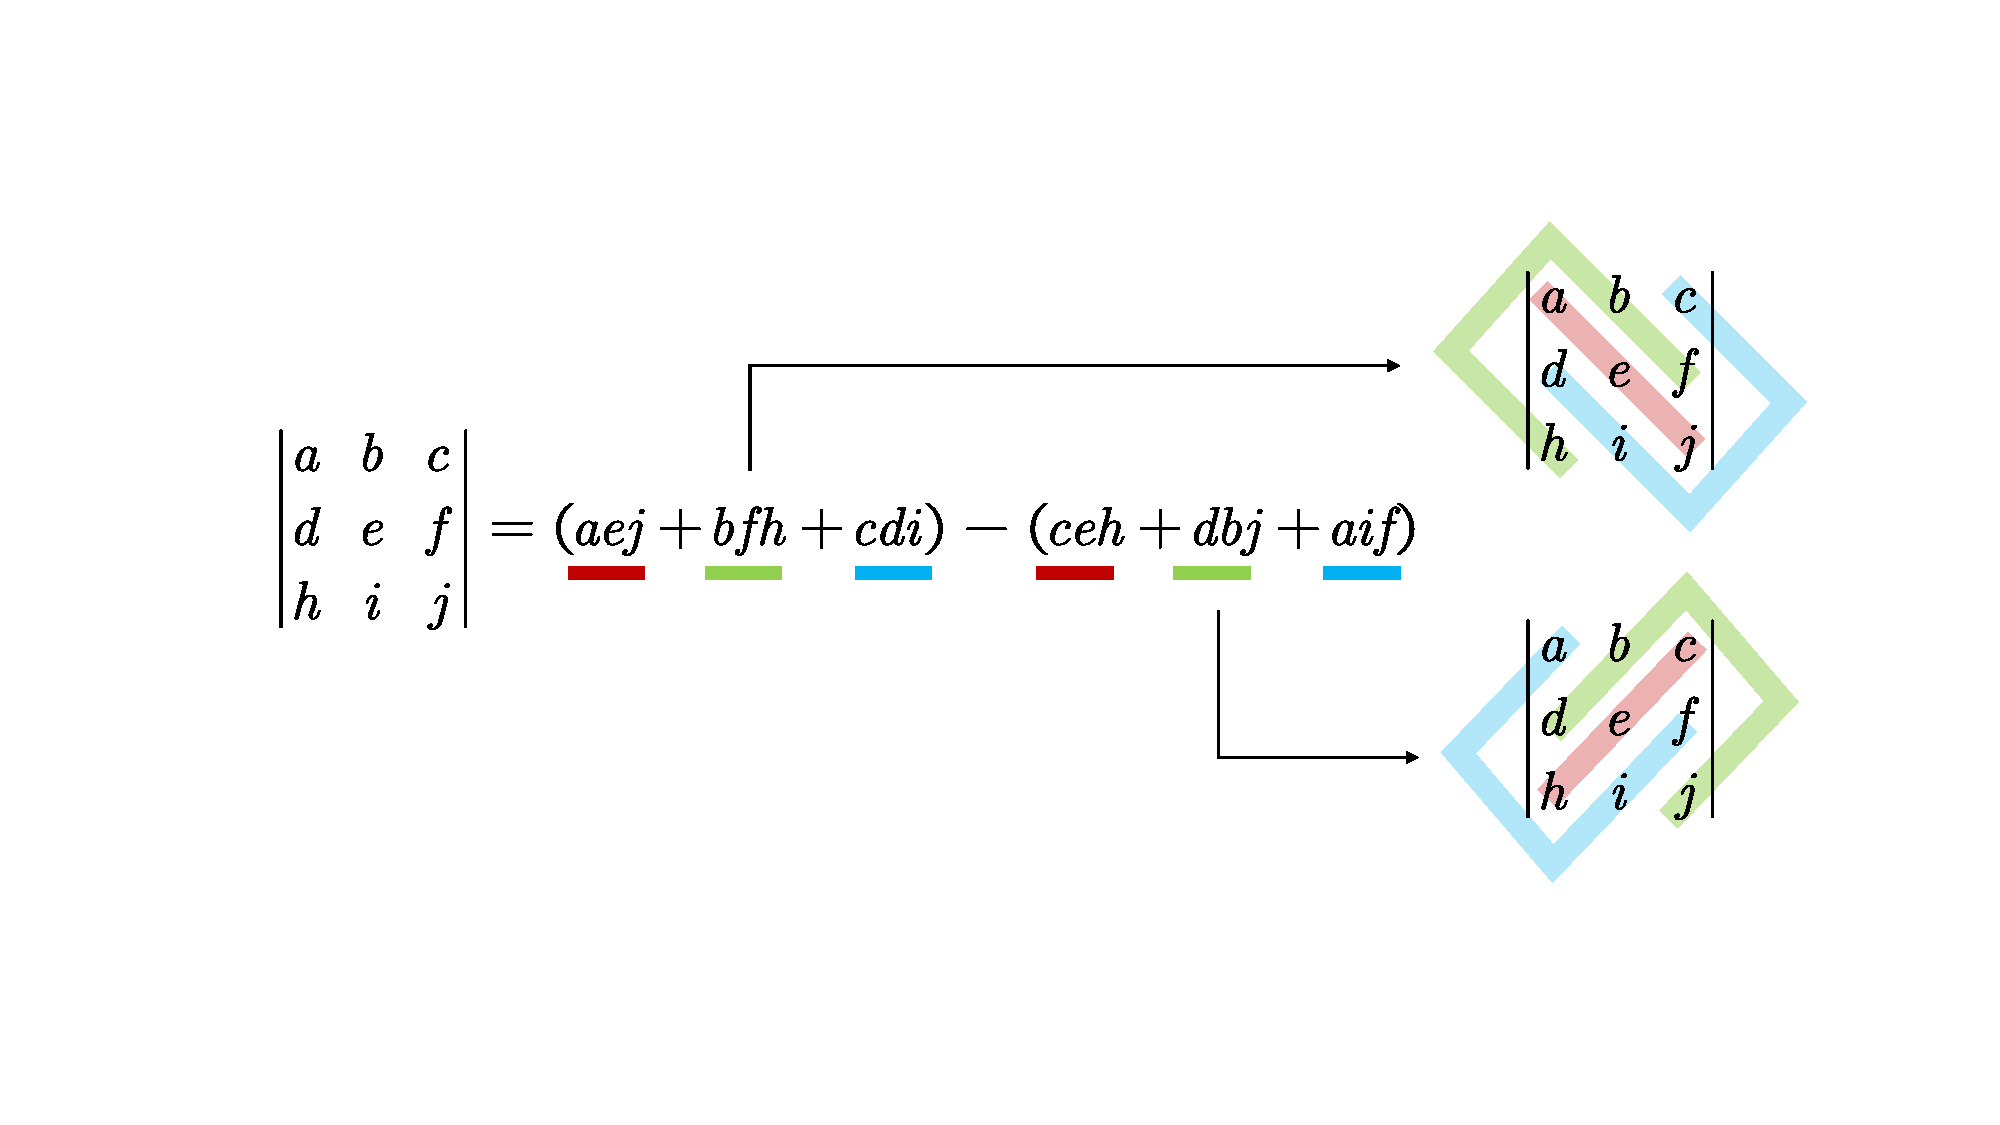
\includegraphics[width=0.8\textwidth]{img/0001.pdf}
	
	
~\\
\hrule
~\\

\section{行列式的几何意义}

\subsection{行列式的值, 表示的是``新基"的面积 ($ \hat{i} × \hat{j}$), 比原基的面积($ i × j$) 大多少倍}

即:
$
\boxed{
	|D| = \frac{ \hat{i} × \hat{j}}{ i × j}
	= \frac{\text{新基的面积}}{\text{原基的面积}}
}$\\


【原基矩阵"的行列式的值】: \\
\begin{align*}
\left| \begin{array}{c|c}
	1&		0\\
	\underset{i}{\underbrace{0}}&		\underset{j}{\underbrace{1}}\\
\end{array} \right|=1*1\ -\ 0*0\ =\underset{=i*j}{\underbrace{1}}\	
\end{align*}

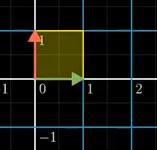
\includegraphics[width=0.2\textwidth]{img/0043.png}\\


【新基矩阵"的行列式的值】: \\

\begin{myEnvSample}
如: 
\begin{align*}
	\left| \begin{array}{c|c}
		3&		2\\
		\underset{i}{\underbrace{0}}&		\underset{j}{\underbrace{2}}\\
	\end{array} \right|=3*2\ -\ 2*0\ =\underset{=i*j}{\underbrace{6}}\
\end{align*}

即, 由``新基"中的两个基向量, 组成的平行四边形的面积 = 6.\\

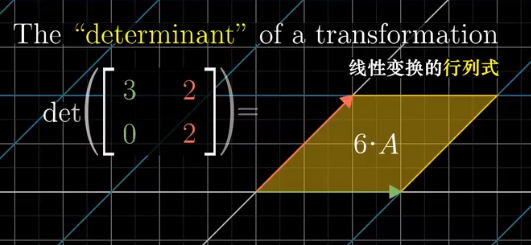
\includegraphics[width=0.6\textwidth]{img/0044.png}
\end{myEnvSample}

所以, 行列式的值, 其几何意义, 本质就是表示: 把原基($i \cdot j$) 这个单元面积, 缩放了多少倍.\\

→ $| D |=3$ : 就意味着, 新基坐标系下, 它已将``原基"的面积 $ (i×j)$, 缩放为了原来的3倍. 即:  $\hat{i} \cdot \hat{j} = 3(i \cdot j) $. \\


→ $| D |=0 $ : 新基矩阵A 里面, 存放的是新基的坐标. 只要 $|A| \ne 0$, 就说明原坐标系空间, 还没有被压缩降维. 那么它就存在 $ A^{-1}$. \\
如果$| D |=0 $ 了, 就意味着, ``原基"已被压缩到一条直线上, 甚至一个点上. 被降维了.\\

→ $|D|=负值 $ : 这意味着, 原坐标系已经被翻转了, 正反面翻转 (invert the orientation of space). 这就被称为``空间定向"发生了改变. 此时, 行列式的值, 就会变成负值.\\


\includegraphics[width=0.35\textwidth]{img/0045.png}

当 i 与 j 越来越靠近, 它们围成的平行四边形的面积, 就越来越小. 即坐标系空间, 被压缩得越来越严重. 当 i 与 j 完全重合时, 它们就共线了, |D| = 0.



~\\
\hrule
~\\

\subsection{在三维空间中, 行列式的值, 表示的就是: 体积的缩放倍数.}

三维空间中, 原基的行列式的值 $= i \cdot j \cdot k = 1 \cdot 1 \cdot 1 = 1$ \\

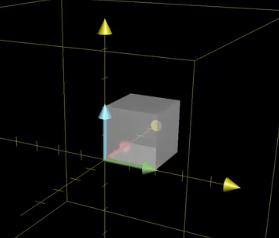
\includegraphics[width=0.2\textwidth]{img/0047.png}\\

在做了变换后, $ |D| = \hat{i} \cdot \hat{j} \cdot \hat{k} $ 会从原立方体, 变为一个斜不拉几的立方体 (即``平行六面体"). after the  transformation, the cube might get wrapped into some kind of slanty cube.\\

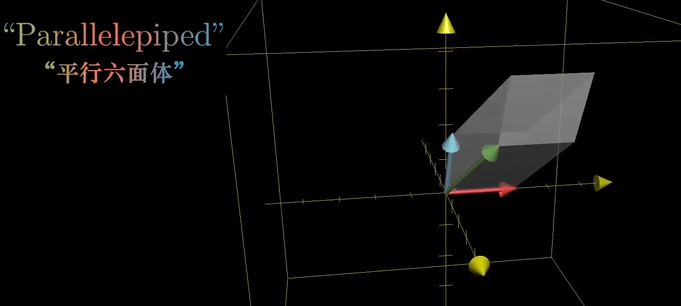
\includegraphics[width=0.6\textwidth]{img/0046.png}\\

三维空间中 : \\
→ $|D|=0$, 就意味着整个空间被压缩成 0体积的东西, 即一个平面, 或一条线, 甚至是一个点. 换言之, 此时的新基$ \hat{i}, \hat{j}, \hat{k}$ 线性相关了.\\
→ 若 |D|是负值, 就意味着整个坐标系的``定向"发生了改变. \\

你可以用``右手螺旋法则" 来确定坐标系的``定向"是否发生了改变.\\





~\\
\hrule
~\\

	
	\section{全排列和对换}
	
	【排列】:\\
	由1,2,...,n 组成的一个``有序"数组, 叫``n级排列".\\
	注意: (1)它是有"顺序"的. 比如: \textbf{1}23, 132, \textbf{2}13, 231, \textbf{3}12, 321.  ← 这个就叫``3级排列".\\
	
	(2)它中间不能缺数, 必须是包含1,2,3...到n的 全部这n个数字, 中间不能缺少任何一个数字. \\
	那么n个数字, 它的全排列(就是排列组合中的排列), 有多少种可能性呢? 那就是: 第1个数字的位置上, 可以从这种n个数字中任取一个出来放. 第二个位置上, 就是从 n-1 的数字中,任取一个出来摆放..., 一共就有: $n\cdot \left( n-1 \right) \cdot \left( n-2 \right) \cdot ...\cdot 3\cdot 2\cdot 1 = n!	$ 种排列方式.\\
	
	
	【逆序】:\\
	``大的数字"排在``小的数字"的前面, 就叫``逆序". 比如: 4213,  4这个大数字, 排在了2这个小数字的前面. \\
	
	
	【逆序数 negative】:\\	
	就是逆序的总数, 你只要数一数有多少个``逆序"存在, 这个总数就是``逆序数".\\
	比如, 4213, 它的逆序有: \\
	- 4后面, 有3个数字比它小 (即2, 1, 3) \\
	- 2后面, 有一个比它小 (即数字1). \\
	- 1后面, 没有比它小的. \\
	- 3后面, 没有比它小的. \\
	所以, 逆序的总数, 就是 3+1+0+0=4 \\
	
	我们用N 来代表``逆序数". 即写成: N(4213)=4 \\
	又如: N(1,2,3,...,n)=0 ← 它也叫``n级标准排列", 或``n级自然排列"\\
	
	\begin{myEnvSample}
	求逆序数: $	N\left( n\cdot \left( n-1 \right) \cdot \left( n-2 \right) \cdot ...\cdot 3\cdot 2\cdot 1 \right) =?	$\\
	数一数: $	\underset{\text{后面有}n-1\text{个比它小的}}{\underbrace{n}}\cdot \underset{\text{后面有}n-2\text{个比它小的}}{\underbrace{\left( n-1 \right) }}\cdot \left( n-2 \right) \cdot ...\cdot 3\cdot \underset{\text{后面有1个比它小的}}{\underbrace{2}}\cdot 1		$ \\
	全加起来就是: $\left( n-1 \right) +\left( n-2 \right) +...+3+2+1=\frac{n\left( n-1 \right)}{2}$个	
	\end{myEnvSample}


	
	【偶排列】:\\
	如果``逆序数N"是偶数, 就是``偶排列". \\
	
	
	【奇排列】:\\
	如果``逆序数N"是奇数, 就是``奇排列".	\\
	
	【对换】:\\
	即交换两个数. 如: 把54\underline{12}3 中的12交换一下, 就变成了 54\underline{21}3 \\
	那么我们来看看它们的逆序数:\\
	- $N\left( \underset{\text{后面有4个比它小的}.}{\underbrace{5}}4\underset{}{\underbrace{1}}\underset{}{\underbrace{2}}3 \right) =4+3+0+0+0=7	$ ← 是奇排列\\
	- $N\left( 54\underset{\text{后面有1个比它小的}}{\underbrace{2}}\underset{}{\underbrace{1}}3 \right) =4+3+1+0+0=8		$ ← 是偶排列\\
	
	所以我们就有定理: \textbf{一个排列中的任意两个元素, 做一次``对换",排列会改变其``奇偶性".} 那么做两次对换呢? 奇偶性又回来了, 即奇偶性就不变了. \\
	
	定理: 在所有的n级排列中(一个``n级排列"的排列数 = n!), 奇排列和偶排列, 各占一半, 即$=\dfrac{n!}{2}$.\\
	
	

	\hrule

	
	\section{n 阶行列式}
	
	\subsection{三阶行列式}
	首先看这个三阶行列式: 
	\begin{align*}
		\begin{matrix}
			\left| \begin{matrix}
				a_{11}&		a_{12}&		a_{13}\\
				a_{21}&		a_{22}&		a_{23}\\
				a_{31}&		a_{22}&		a_{33}\\
			\end{matrix} \right|\\
			=a_{11}a_{22}a_{33}+a_{12}a_{23}a_{31}+a_{13}a_{21}a_{32}\\
			-a_{13}a_{22}a_{31}-a_{12}a_{21}a_{33}-a_{11}a_{23}a_{32}\\
		\end{matrix}
	\end{align*} 
	等号右边: \\
	- 每一项的``行标"( 六项各自的行标, 分别是: 123, 123, 123, 123, 123, 123), 取的是``标准排列".	\\
	- \textbf{``列标": 取``排列的所有可能"(即所有可能的排列顺序, 都取到了). 比如, 4阶行列式, 有4列, 那么4个数字的全排列的总数= 4!=24种不同的排序. 即这个4阶行列式展开后, 共有24项.}  即: \\
	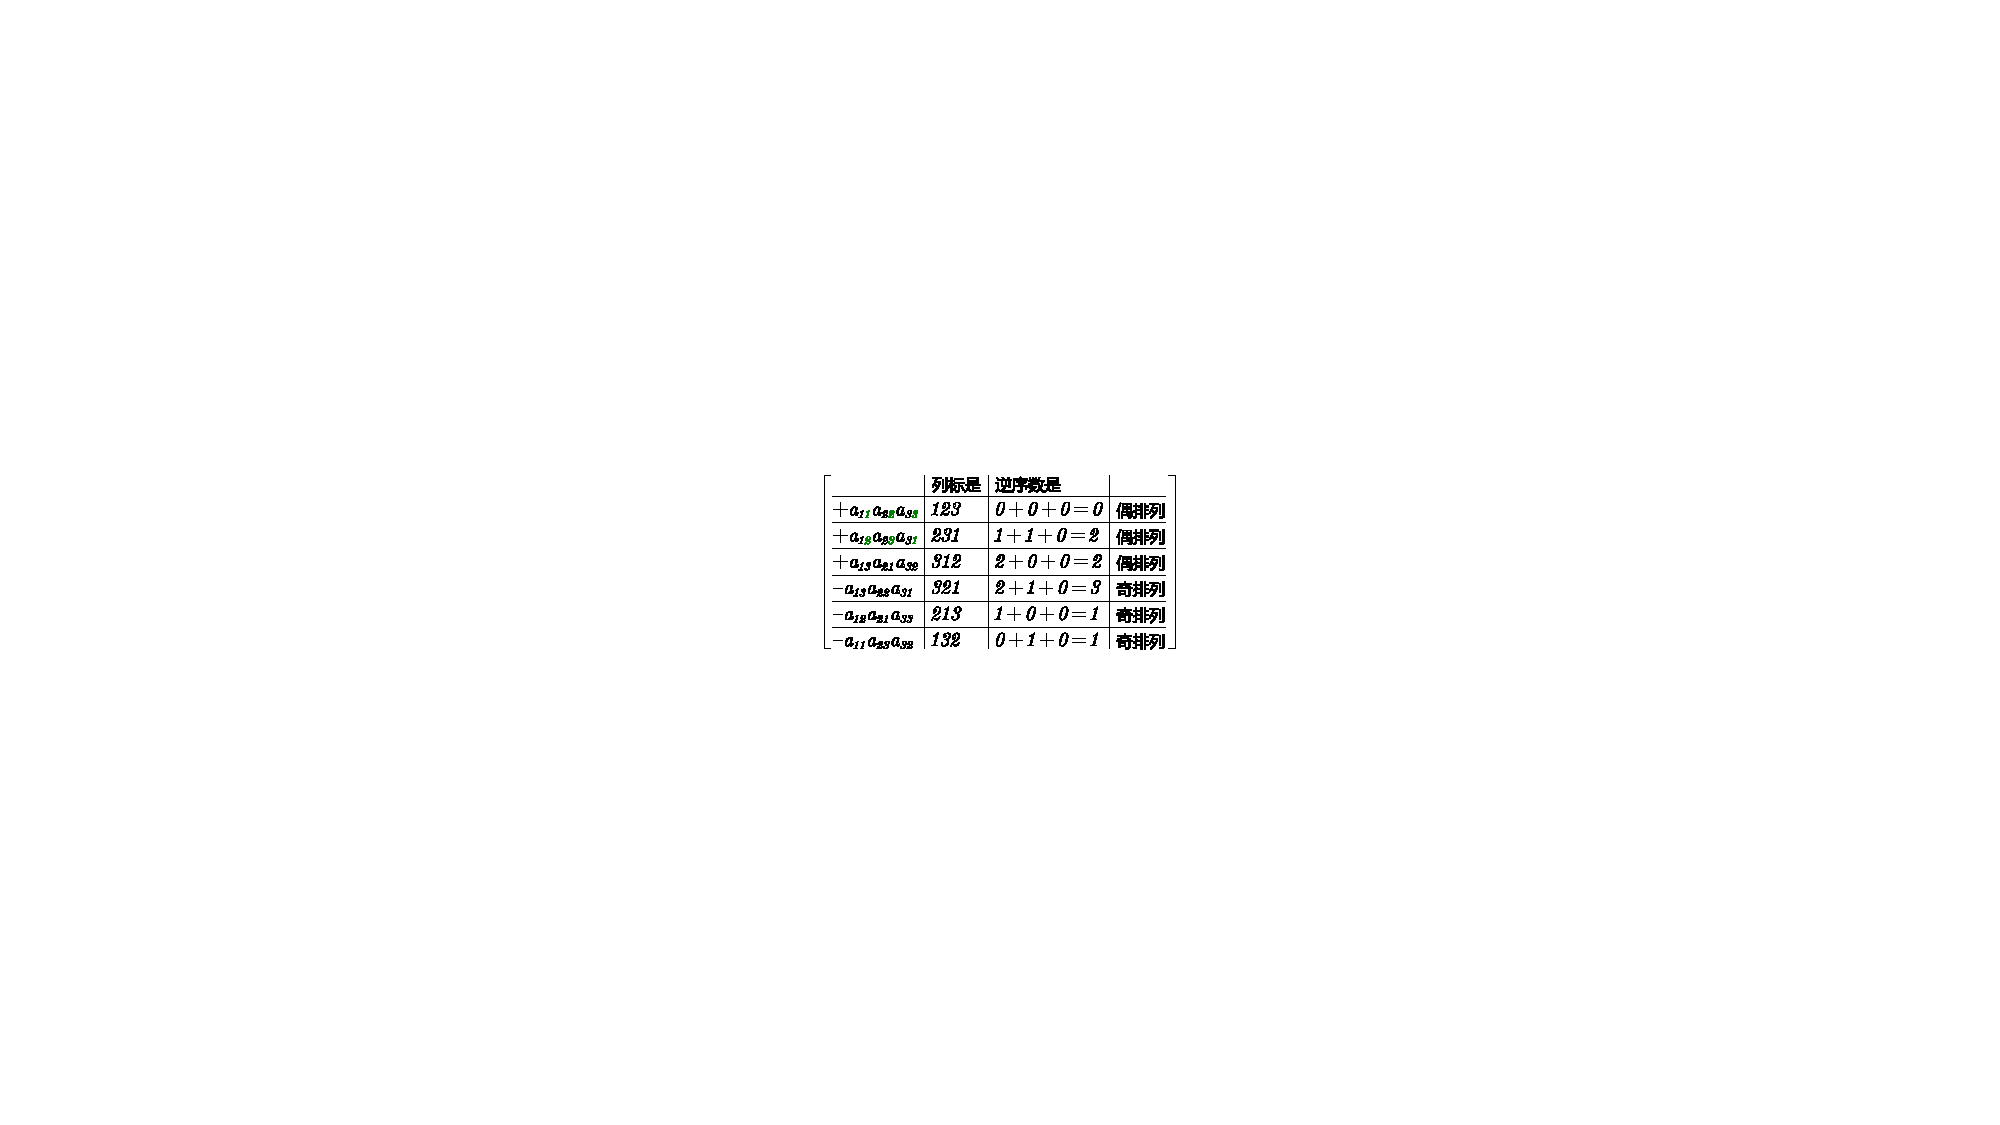
\includegraphics[width=0.5\textwidth]{img/0002.pdf}\\
	
	可以看出: 各项前的正负符号, 是由``列标"的奇偶性(奇排列还是偶排列)决定的 (奇负, 偶正).\\
	- 每一项, 就是从这个行列式的``不同行, 不同列"中, 取出3个元素, 来相乘.\\
	
	上面这个, 即``n阶行列式"的第一种定义方式. 也就是``按行展开".\\
	
	

	\hrule

	
	
	\subsection{n 阶行列式 -- 按行展开}
	
	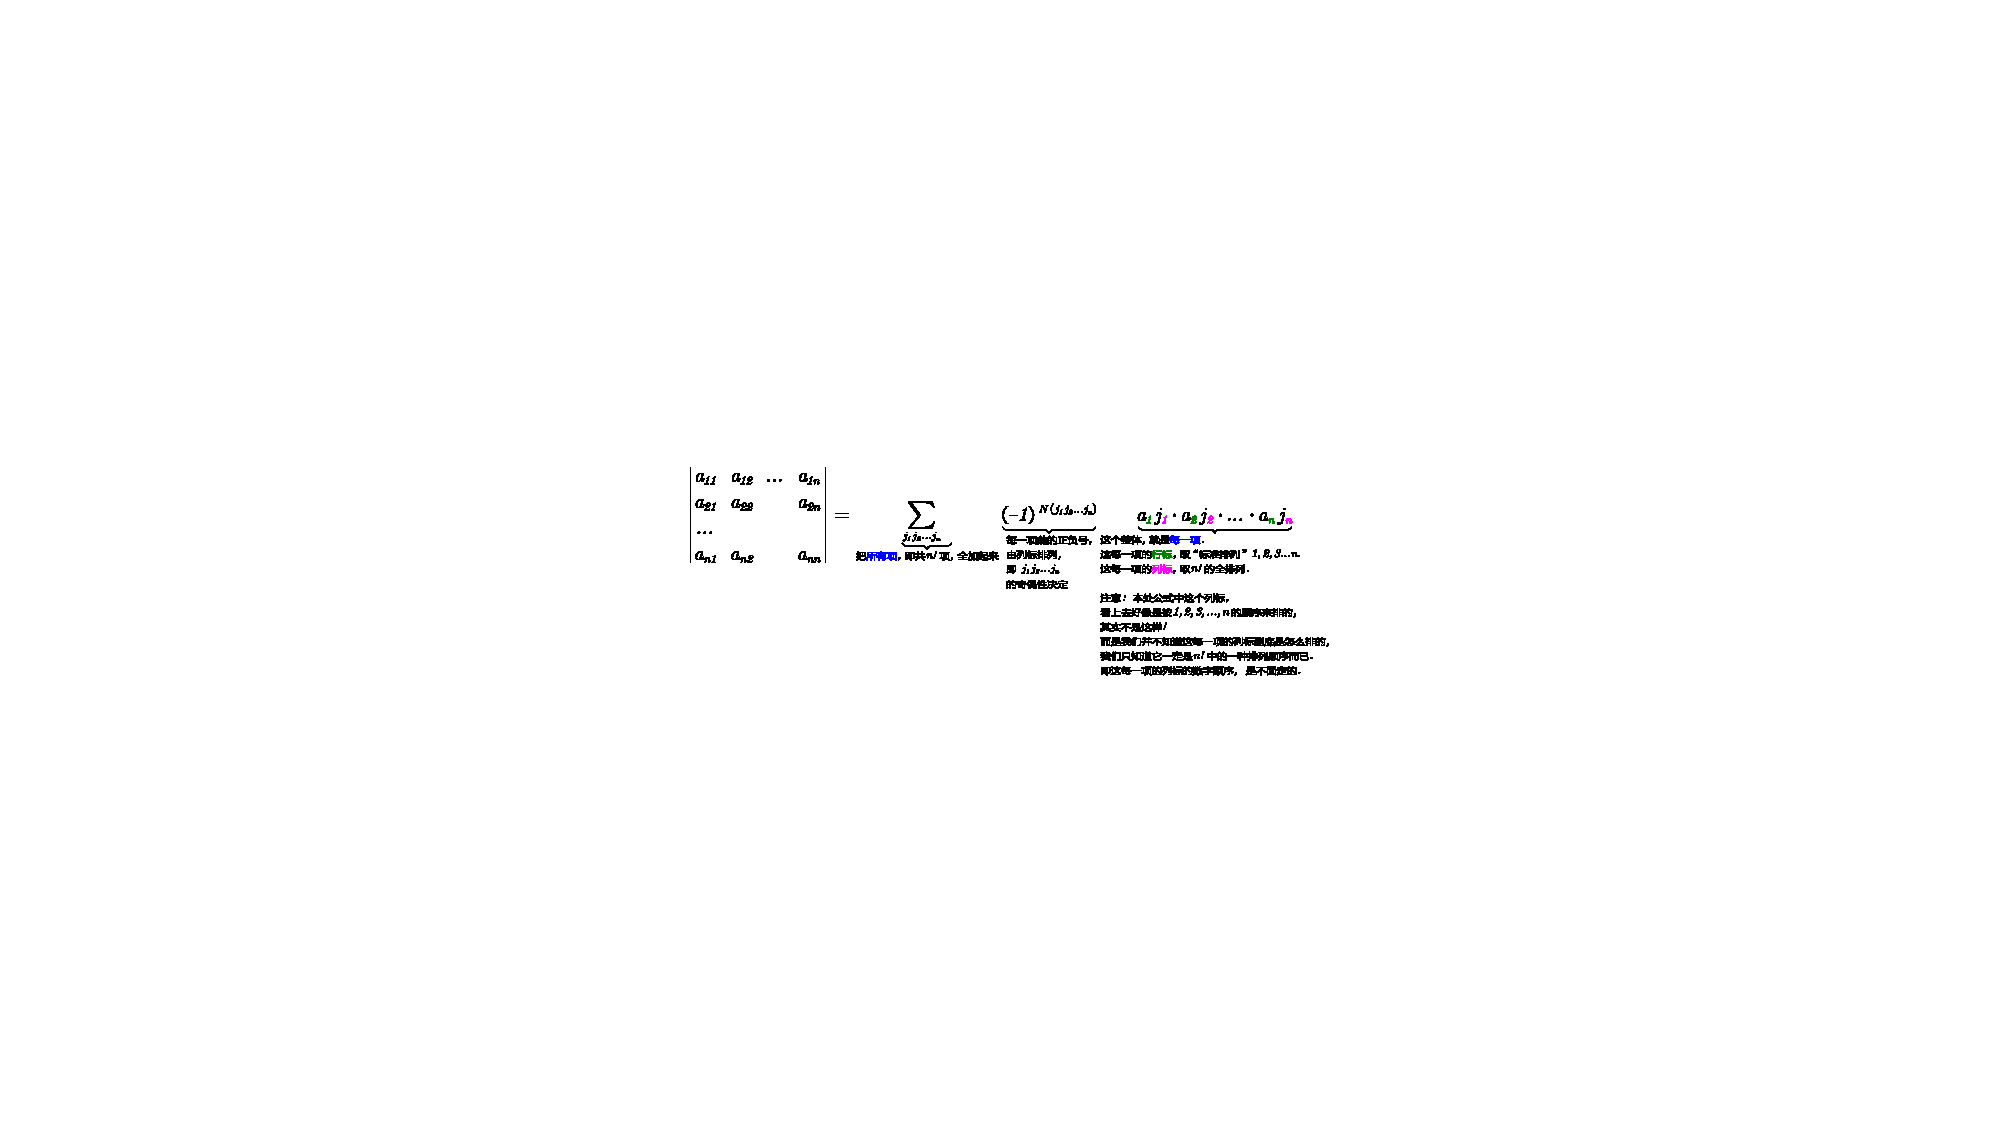
\includegraphics[width=1\textwidth]{img/0003.pdf}\\
	
	n阶行列式的展开, 一共有多少项呢? 共有 n! 项. \\
	
	行列式, 用 D (determinant) 来表示. 写成: $	D=\left| a_{ij} \right|	$
	
	\begin{myEnvSample}
	determinant : n. ( formal ) a thing that decides whether or how sth happens 决定因素;决定条件
	\end{myEnvSample}

	只有一个元素的行列式, 就等于该元素本身, 即:	$	\left| a_{11} \right|=a_{11}	$\\
	|8|=8\\
	|-1|=-1\\
	
	\begin{myEnvSample}
$
\left| \begin{matrix}
	&		2&		&		\\
	&		&		3&		\\
	&		&		&		4\\
	1&		&		&		\\
\end{matrix} \right|=\left( -1 \right) ^{N\left( 2341 \right)}\ 2\cdot 3\cdot 4\cdot 1=-24
$
	\end{myEnvSample}
	


\hrule

	
\subsubsection{下三角行列式 =主对角线上元素的乘积}

$
\underset{\text{下三角行列式}}{\underbrace{\left| \begin{matrix}
			a_{11}&		&		&	0	\\
			a_{21}&		a_{22}&		&		\\
			...&		&		...&		\\
			a_{n1}&		...&		...&		a_{nn}\\
		\end{matrix} \right|}}=\underset{\text{即主对角线元素相乘}}{\underbrace{a_{11}\cdot a_{22}\cdot ...\cdot a_{nn}}}
$


\hrule


\subsubsection{上三角行列式 =主对角线上元素的乘积}

$
\underset{\text{上三角行列式}}{\underbrace{\left| \begin{matrix}
			a_{11}&		...&		&		a_{1n}\\
			&		a_{22}&		&		a_{2n}\\
			&		&		...&		...\\
			0&		&		&		a_{nn}\\
		\end{matrix} \right|}}=\underset{\text{即主对角线元素相乘}}{\underbrace{a_{11}\cdot a_{22}\cdot ...\cdot a_{nn}}}
$\\



\hrule


\subsubsection{对角形行列式 =主对角线上元素的乘积}
$
\underset{\text{对角形行列式}}{\underbrace{\left| \begin{matrix}
			a_{11}&		&		&		0\\
			&		a_{22}&		&		\\
			&		&		...&		\\
			0&		&		&		a_{nn}\\
		\end{matrix} \right|}}=\underset{\text{即主对角线元素相乘}}{\underbrace{a_{11}\cdot a_{22}\cdot ...\cdot a_{nn}}}
$\\

\hrule

\subsubsection{伪下三角行列式  $	=\left( -1 \right) ^{\frac{n\left( n-1 \right)}{2}}a_{1,n}\cdot a_{2,n-1}\cdot a_{n,1}	$}

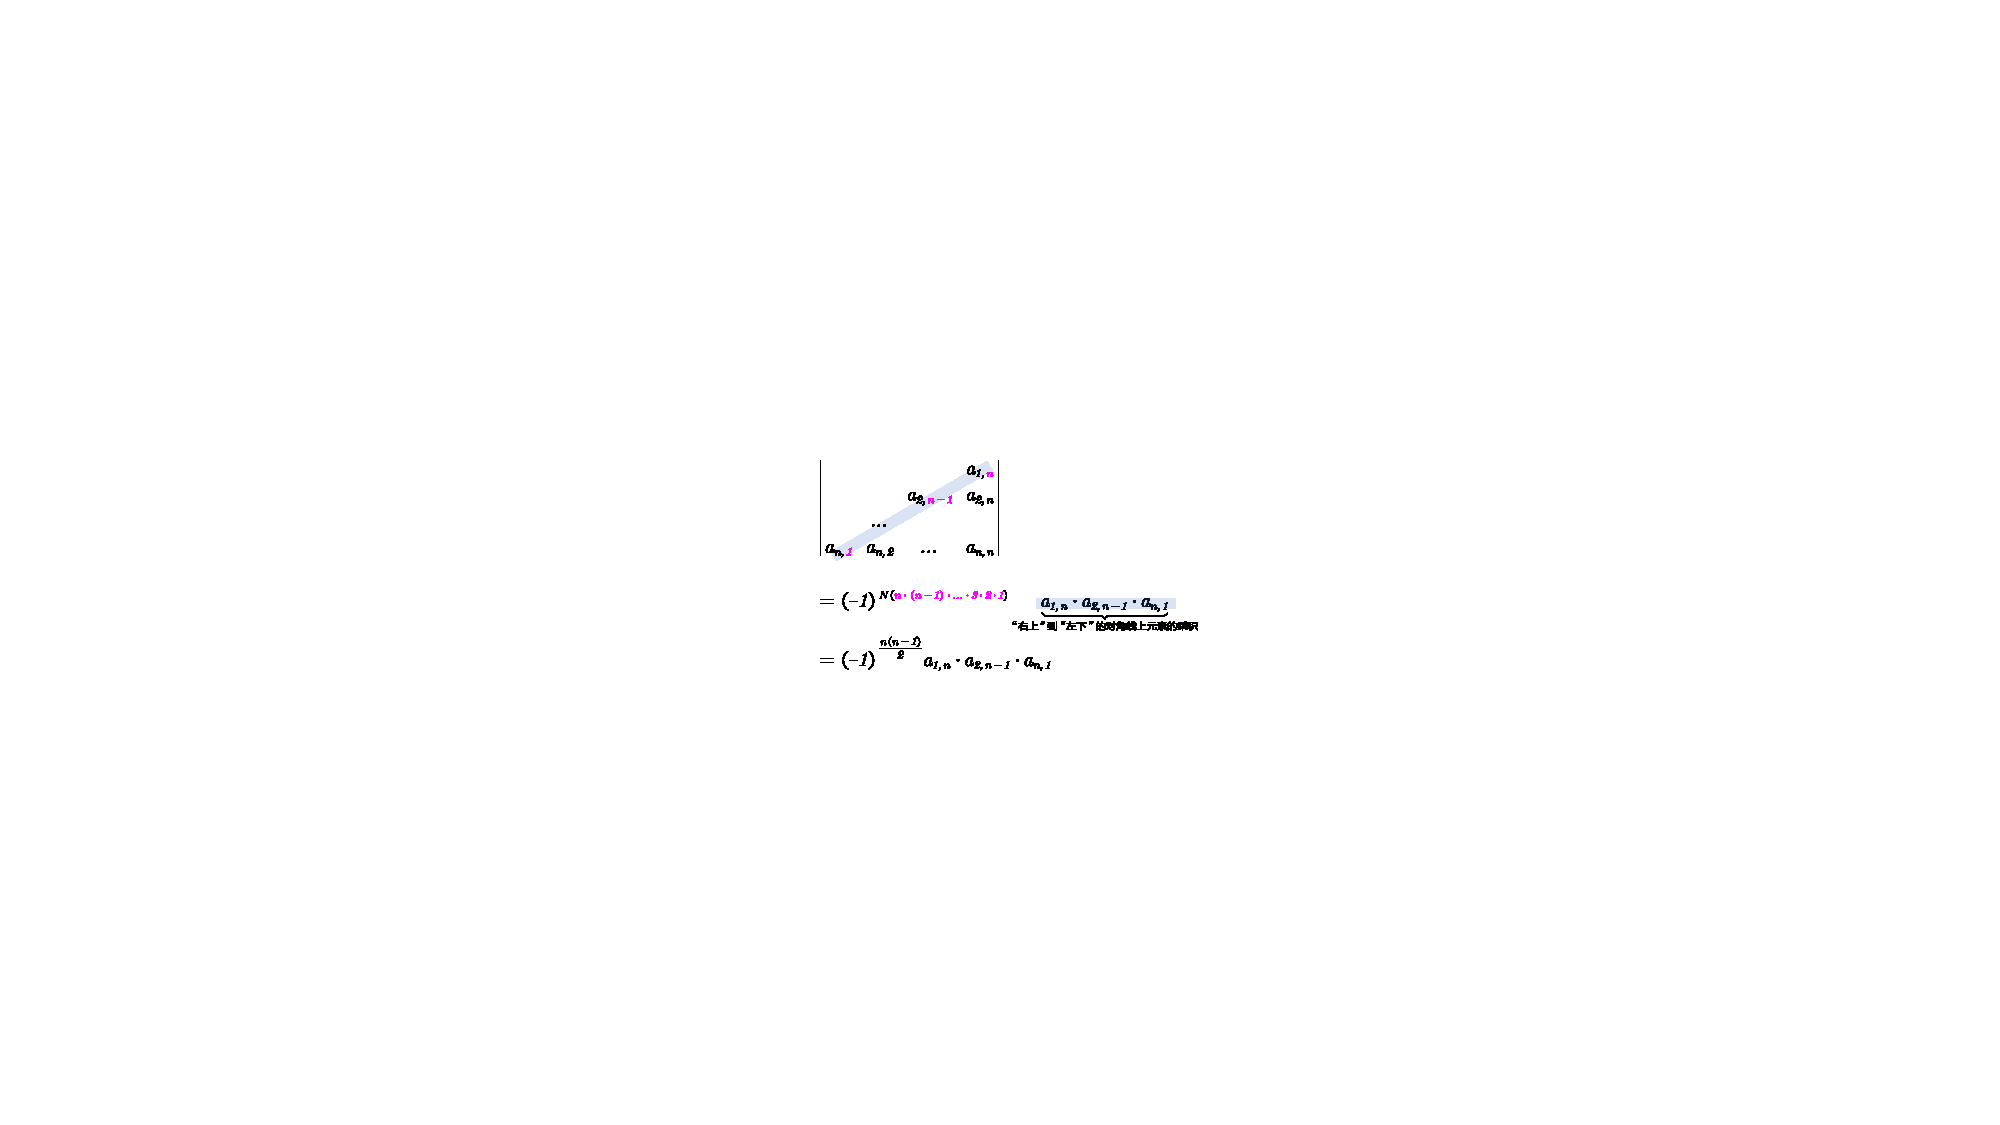
\includegraphics[width=0.6\textwidth]{img/0004.pdf}\\



\hrule


\subsubsection{伪上三角行列式 $	=\left( -1 \right) ^{\frac{n\left( n-1 \right)}{2}}a_{1,n}\cdot a_{2,n-1}\cdot a_{n,1}	$}

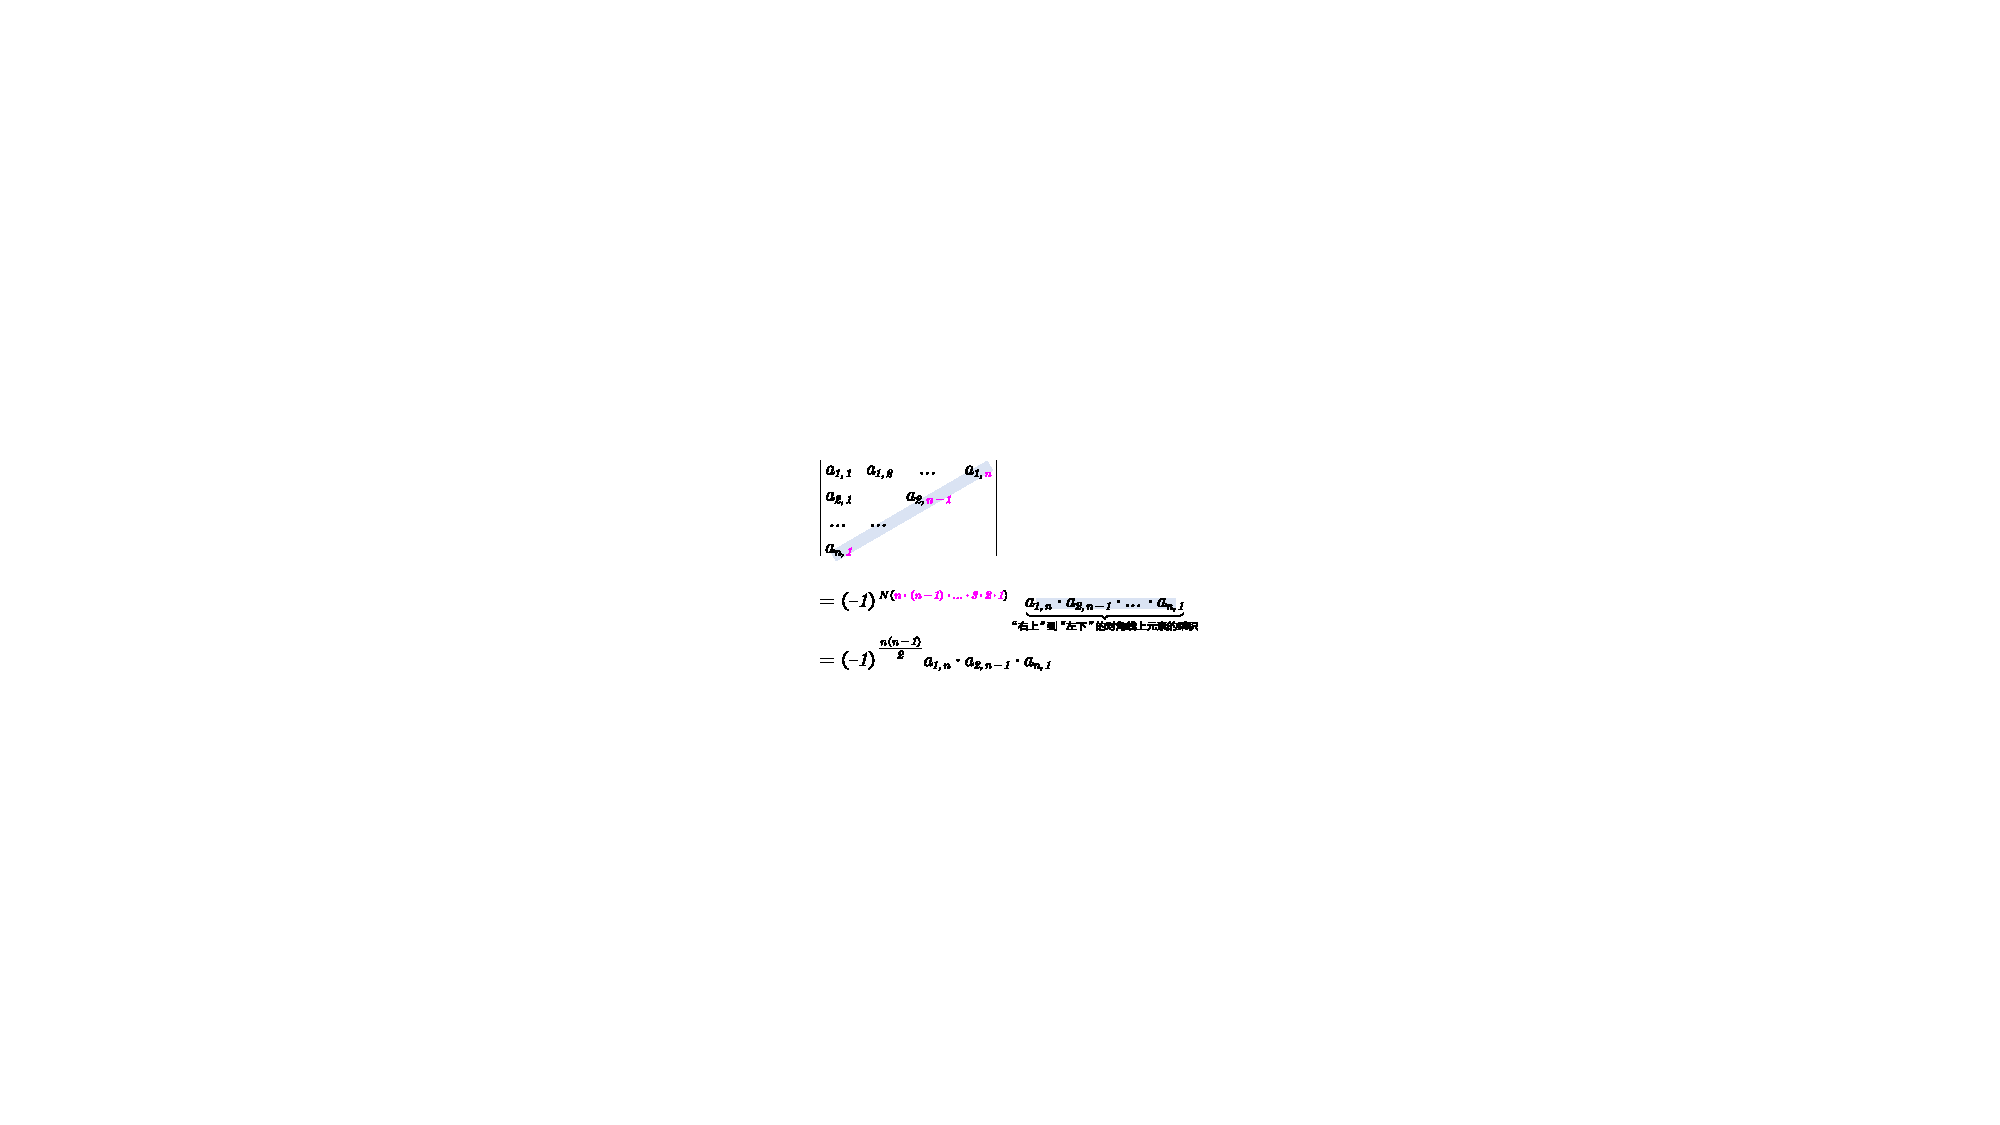
\includegraphics[width=0.6\textwidth]{img/0005.pdf}\\



\hrule


	\subsection{n 阶行列式 -- 按列展开} 
	
	【行列式, 按列展开】:\\
	- ``列标"取自然排列 1,2,3,...,n.  \\
	- ``行标"取n个数的``全排列"的所有排序可能. \\
	- 从不同行, 不同列, 取n个元素来相乘, 就得到每一项. \\
	- 每一项前的正负号, 由``行标排列"的``奇偶性"来决定. \\
	
	行列式``按列展开"的公式即: \\
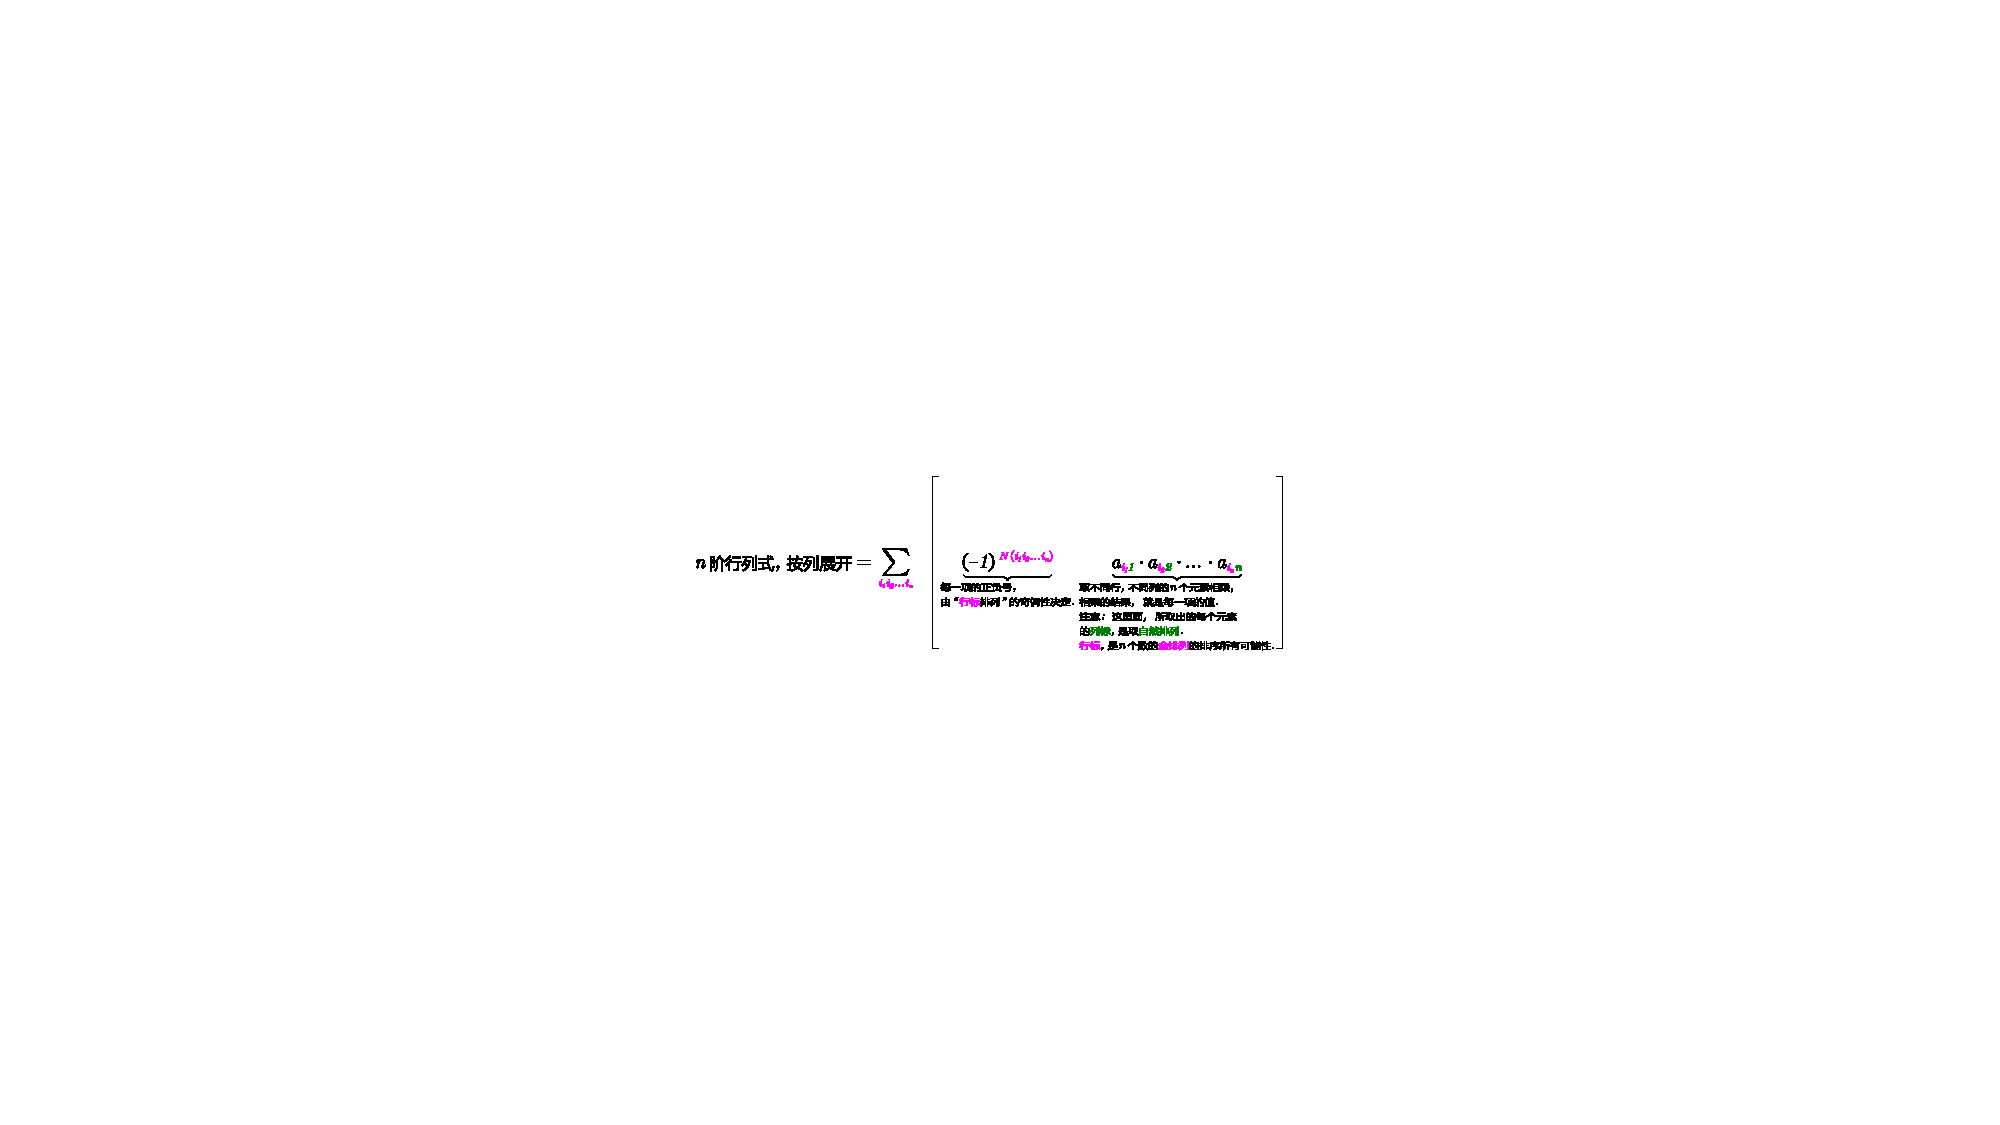
\includegraphics[width=1\textwidth]{img/0006.pdf}\\


\hrule

	
	
	\section{行列式的性质}
	
	【行列式的转置 transpose】:\\
	转置, 就是, 行变列, 或列变行. 如:\\
	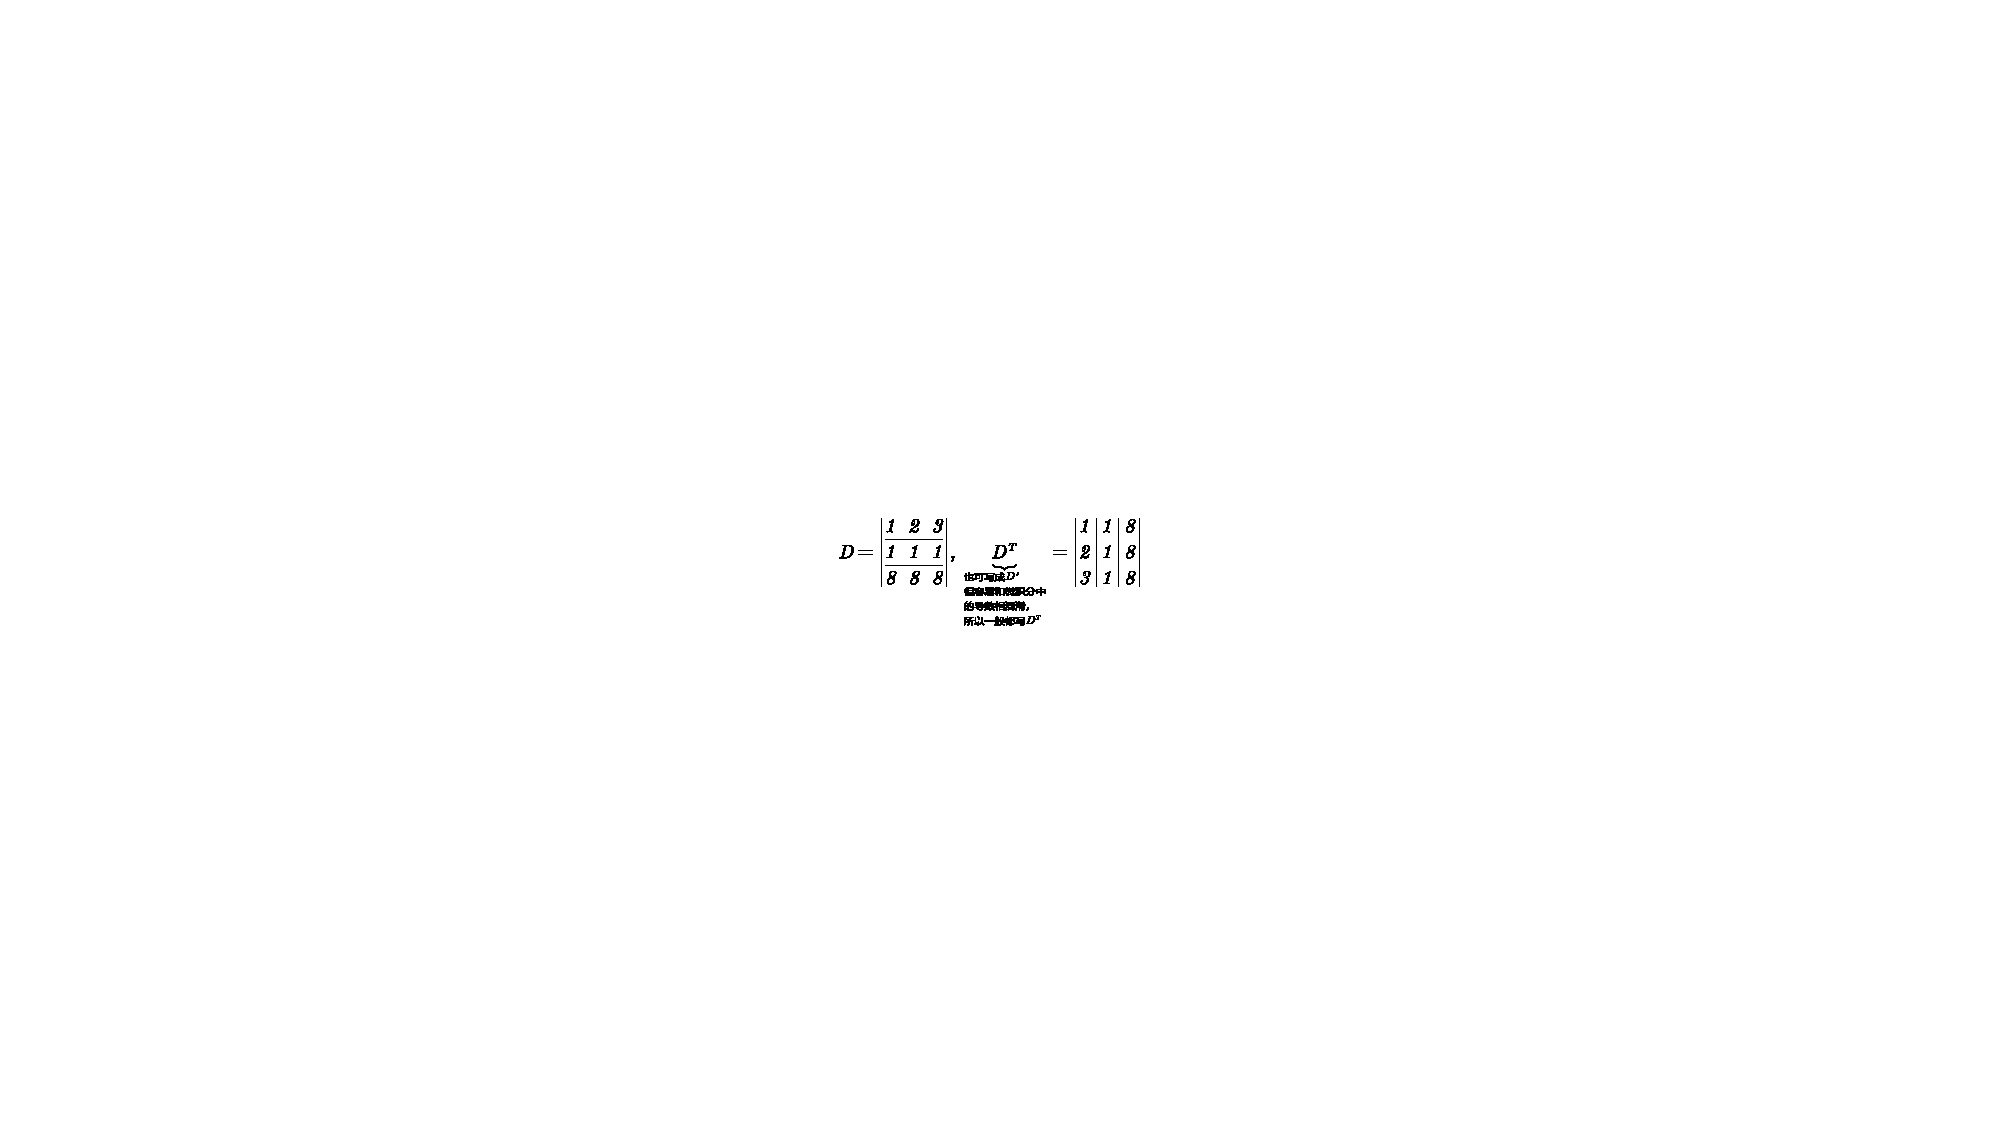
\includegraphics[width=0.45\textwidth]{img/0007.pdf}\\
	
	
	
	\subsection{性质: $\left( D^T \right) ^T=D$	}
	
	
	\hrule
	
	\subsection{性质: $D^T=D$ }
	\textbf{行列式转置与否, 其值不变.} \\
	\textbf{对``行"成立的性质, 对``列"也成立.} \\
	
\hrule
	
	\subsection{性质: 行列式中两行(两列也行)互换, 行列式的值, 就改变正负号 }
	
	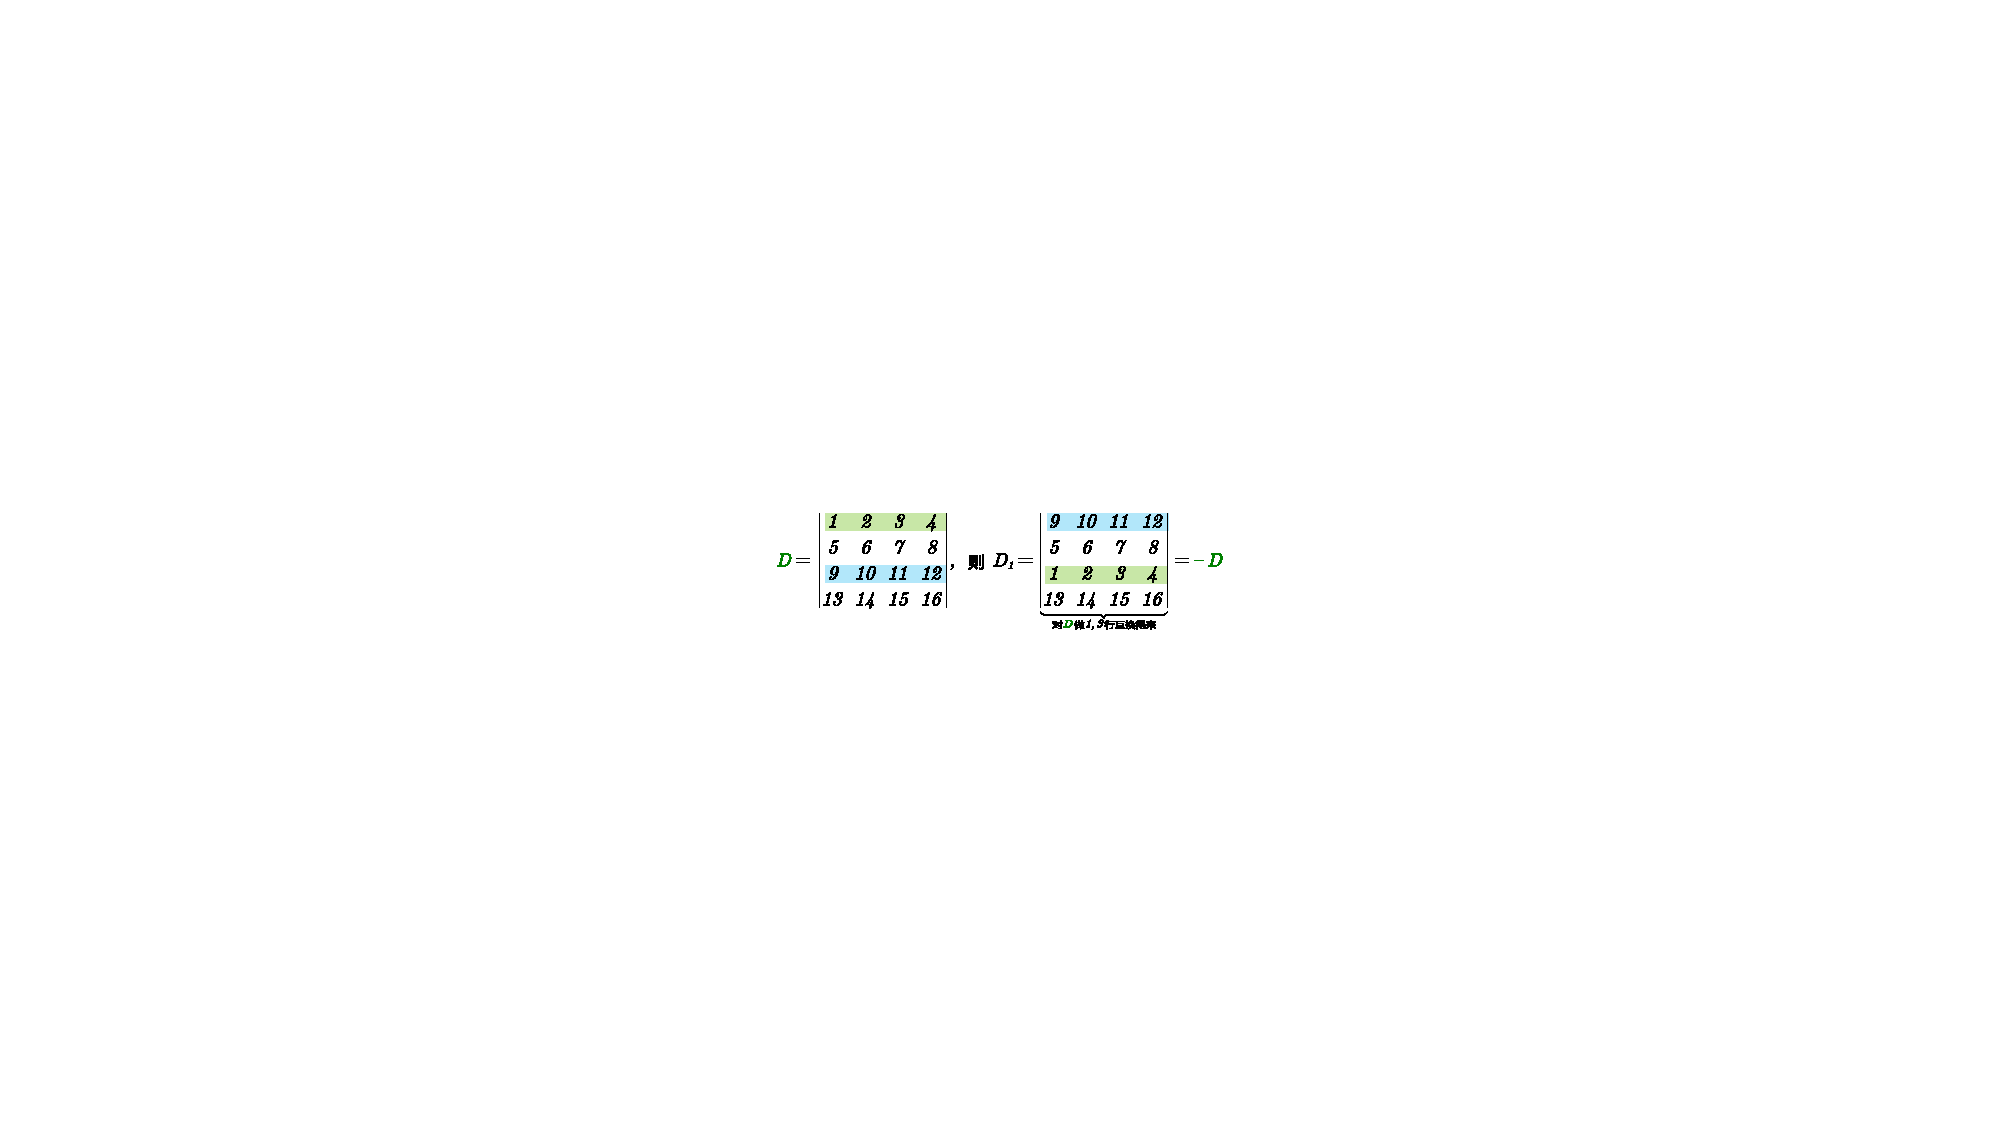
\includegraphics[width=0.6\textwidth]{img/0008.pdf}\\
	
	\hrule
	
	\subsection{性质: 行列式, 若两行(或两列)的元素相等, 则该行列式的值=0}
	
	有这个行列式, 其第1,3行上的元素, 完全相同. \\
	$
	D=\left| \begin{matrix}
		2&		3&		4&		5\\
		1&		0&		0&		0\\
		2&		3&		4&		5\\
		8&		8&		8&		1\\
	\end{matrix} \right|
	$ \\
	
	我们对它的1,3行做交换, 得到的$D_1 = -D$ (因为交换两行, 行列式的值要变号). 而新的$D_1$的内容, 和老D依然是完全一样的. 于是我们就有: D=-D, 即2D=0, 即D=0. \\	
	于是我们就得到了这个性质: 行列式, \textbf{若两行(或两列)的元素相等, 则该行列式的值=0.}\\
	
	\hrule
	
	\subsection{性质: 某一行都乘以k, 等于用k乘以这个行列式D }
	即:\\
	$
	\left| \begin{matrix}
		1&		2&		3\\
		4k&		5k&		6k\\
		7&		8&		9\\
	\end{matrix} \right|=k\left| \begin{matrix}
		1&		2&		3\\
		4&		5&		6\\
		7&		8&		9\\
	\end{matrix} \right|
	$\\
	
	换言之就是: \textbf{如果行列式中的某行, 有公因子k, 则k可以提到行列式外面去.} \\
	
	如果每行都有k, 则每行都要提一次k. 比如一共有3行, 就提3次k. \\
	$
	\left| \begin{matrix}
		1k&		2k&		3k\\
		4k&		5k&		6k\\
		7k&		8k&		9k\\
	\end{matrix} \right|=k^3\left| \begin{matrix}
		1&		2&		3\\
		4&		5&		6\\
		7&		8&		9\\
	\end{matrix} \right|
	$ \\
	
	即: 如果一个n阶行列式的所有元素, 均有公因子k, 则k就向外提n次(因为有n行, 每行只需提一次, 就是提n行次). \\
		
	\hrule
	
	\subsection{性质: 行列式的两行(或两列)元素, 对应成比例, 则该行列式的值=0}

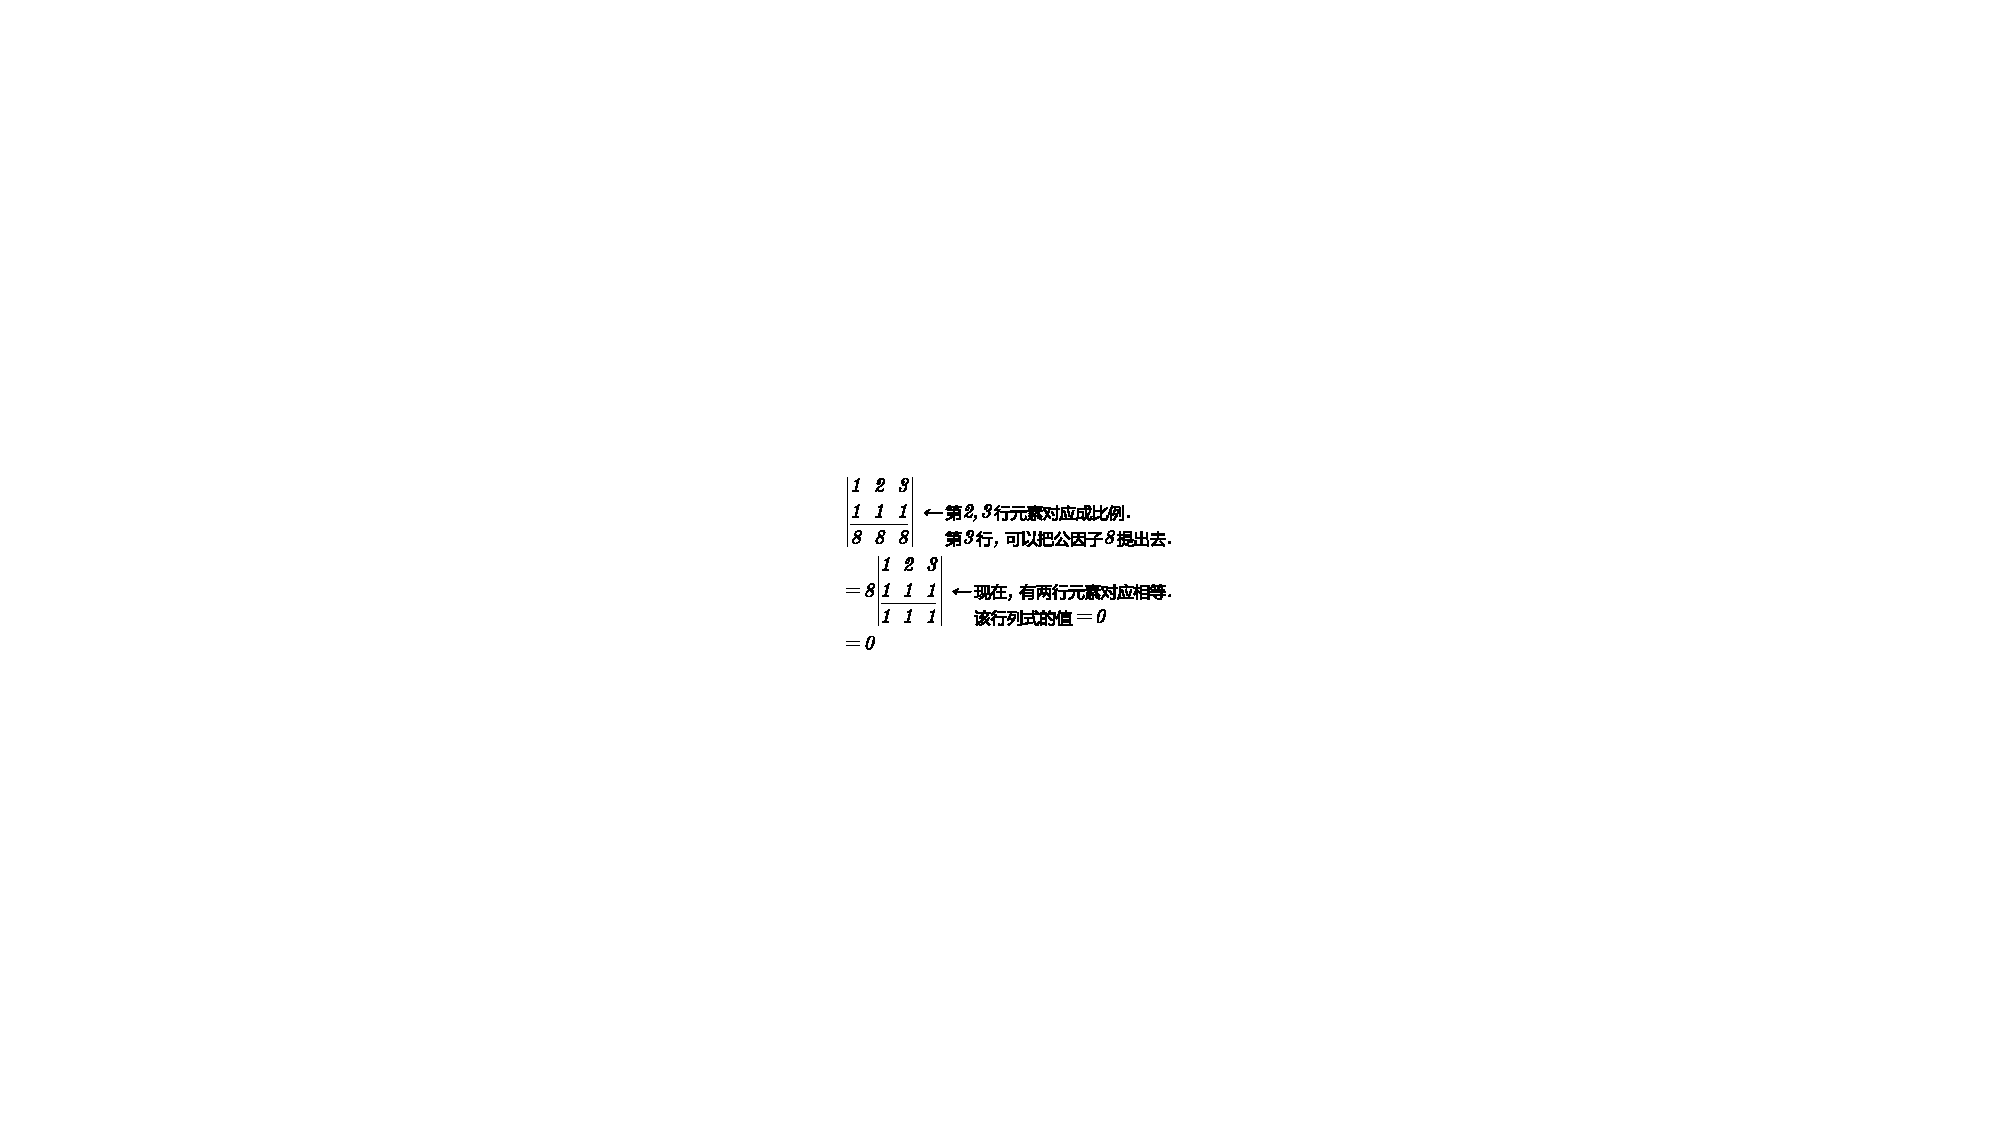
\includegraphics[width=0.45\textwidth]{img/0009.pdf}\\
	
	\hrule
	
	
	\subsection{性质: 某一行全为0, 则D=0 }
	现在, 我们就有了: \\
	
	$
	\left. \begin{array}{r}
		\text{两行上的元素,对应成比例}\\
		\text{某一行元素,全为}0\\
		\text{两行相等}\\
	\end{array} \right\} \ →\ \text{则\ }D=0
	$\\
	
	上面, 左边可以推导出右边. 但反过来, 右边是无法推导出左边的. 即 D=0 的行列式, 未必是属于左边的三种情况之一. \\
	
	\hrule
	
	\subsection{性质: 某一行上的元素, 是两个元素的和的话, 则该行列式就可以拆成这两个行列式相加}
	即:\\
	$
	\left| \begin{matrix}
		1&		2&		3\\
		7+8&		2+3&		9+10\\
		8&		8&		9\\
	\end{matrix} \right|=\ \left| \begin{matrix}
		1&		2&		3\\
		7&		2&		9\\
		8&		8&		9\\
	\end{matrix} \right|+\left| \begin{matrix}
		1&		2&		3\\
		8&		3&		10\\
		8&		8&		9\\
	\end{matrix} \right|
	$\\
	
	注意: 拆分的时候, 只能拆``是和那一行", 其他行的元素要保持不变! 如:\\	
	$
	\left| \begin{matrix}
		b+c&		c+a&		a+b\\
		a+b&		b+c&		c+a\\
		c+a&		a+b&		b+c\\
	\end{matrix} \right|\ne \left| \begin{matrix}
		b&		c&		a\\
		a&		b&		c\\
		c&		a&		b\\
	\end{matrix} \right|+\left| \begin{matrix}
		c&		a&		b\\
		b&		c&		a\\
		a&		b&		c\\
	\end{matrix} \right|\ ←\text{这种拆分是错的!}
	$\\
	
	
	正确的拆分是如下 (比如拆第一行的话): \\	
	$
	\left| \begin{matrix}
		b+c&		c+a&		a+b\\
		a+b&		b+c&		c+a\\
		c+a&		a+b&		b+c\\
	\end{matrix} \right|\ne \left| \begin{matrix}
		b&		c&		a\\
		a+b&		b+c&		c+a\\
		c+a&		a+b&		b+c\\
	\end{matrix} \right|+\left| \begin{matrix}
		c&		a&		b\\
		a+b&		b+c&		c+a\\
		c+a&		a+b&		b+c\\
	\end{matrix} \right|
	$ \\
	
	\hrule
	
	\subsection{ \ding{72} 性质:  某一行乘以一个数, 加到另一行上去, 行列式D的值不变}
	
	\begin{align*}
			& D=\left| \begin{matrix}
				1&		2&		3\\
				1&		1&		0\\
				9&		9&		10\\
			\end{matrix} \right|\ ←\text{将第一行}×5,\text{加到第二行上去}\\
			& =\left| \begin{matrix}
				1&		2&		3\\
				1+\left( 1\cdot 5 \right)&		1+\left( 2\cdot 5 \right)&		0+\left( 3\cdot 5 \right)\\
				9&		9&		10\\
			\end{matrix} \right|\\
			& =\left| \begin{matrix}
				1&		2&		3\\
				1+5&		1+10&		0+15\\
				9&		9&		10\\
			\end{matrix} \right|\ ←\text{第二行的元素是两个数的和,\ 可以拆分成两个行列式}\\
			& =\left| \begin{matrix}
				1&		2&		3\\
				1&		1&		0\\
				9&		9&		10\\
			\end{matrix} \right|+\underset{\text{第1,2行成比例,\ 这个行列式的值}=0}{\underbrace{\left| \begin{matrix}
						1&		2&		3\\
						5&		10&		15\\
						9&		9&		10\\
					\end{matrix} \right|}}\\
			& =\left| \begin{matrix}
				1&		2&		3\\
				1&		1&		0\\
				9&		9&		10\\
			\end{matrix} \right|=D
	\end{align*}
	
	
	
	\hrule
	
	
	\section{行列式值的计算 }
	
	\subsection{方法是: 把行列式, 先化成``上三角行列式"}
	
	方法论: 一般, 我们要把行列式, 化成``上三角行列式". 则该行列式的值, 就是``主对角线"上元素的乘积了. \\
	
	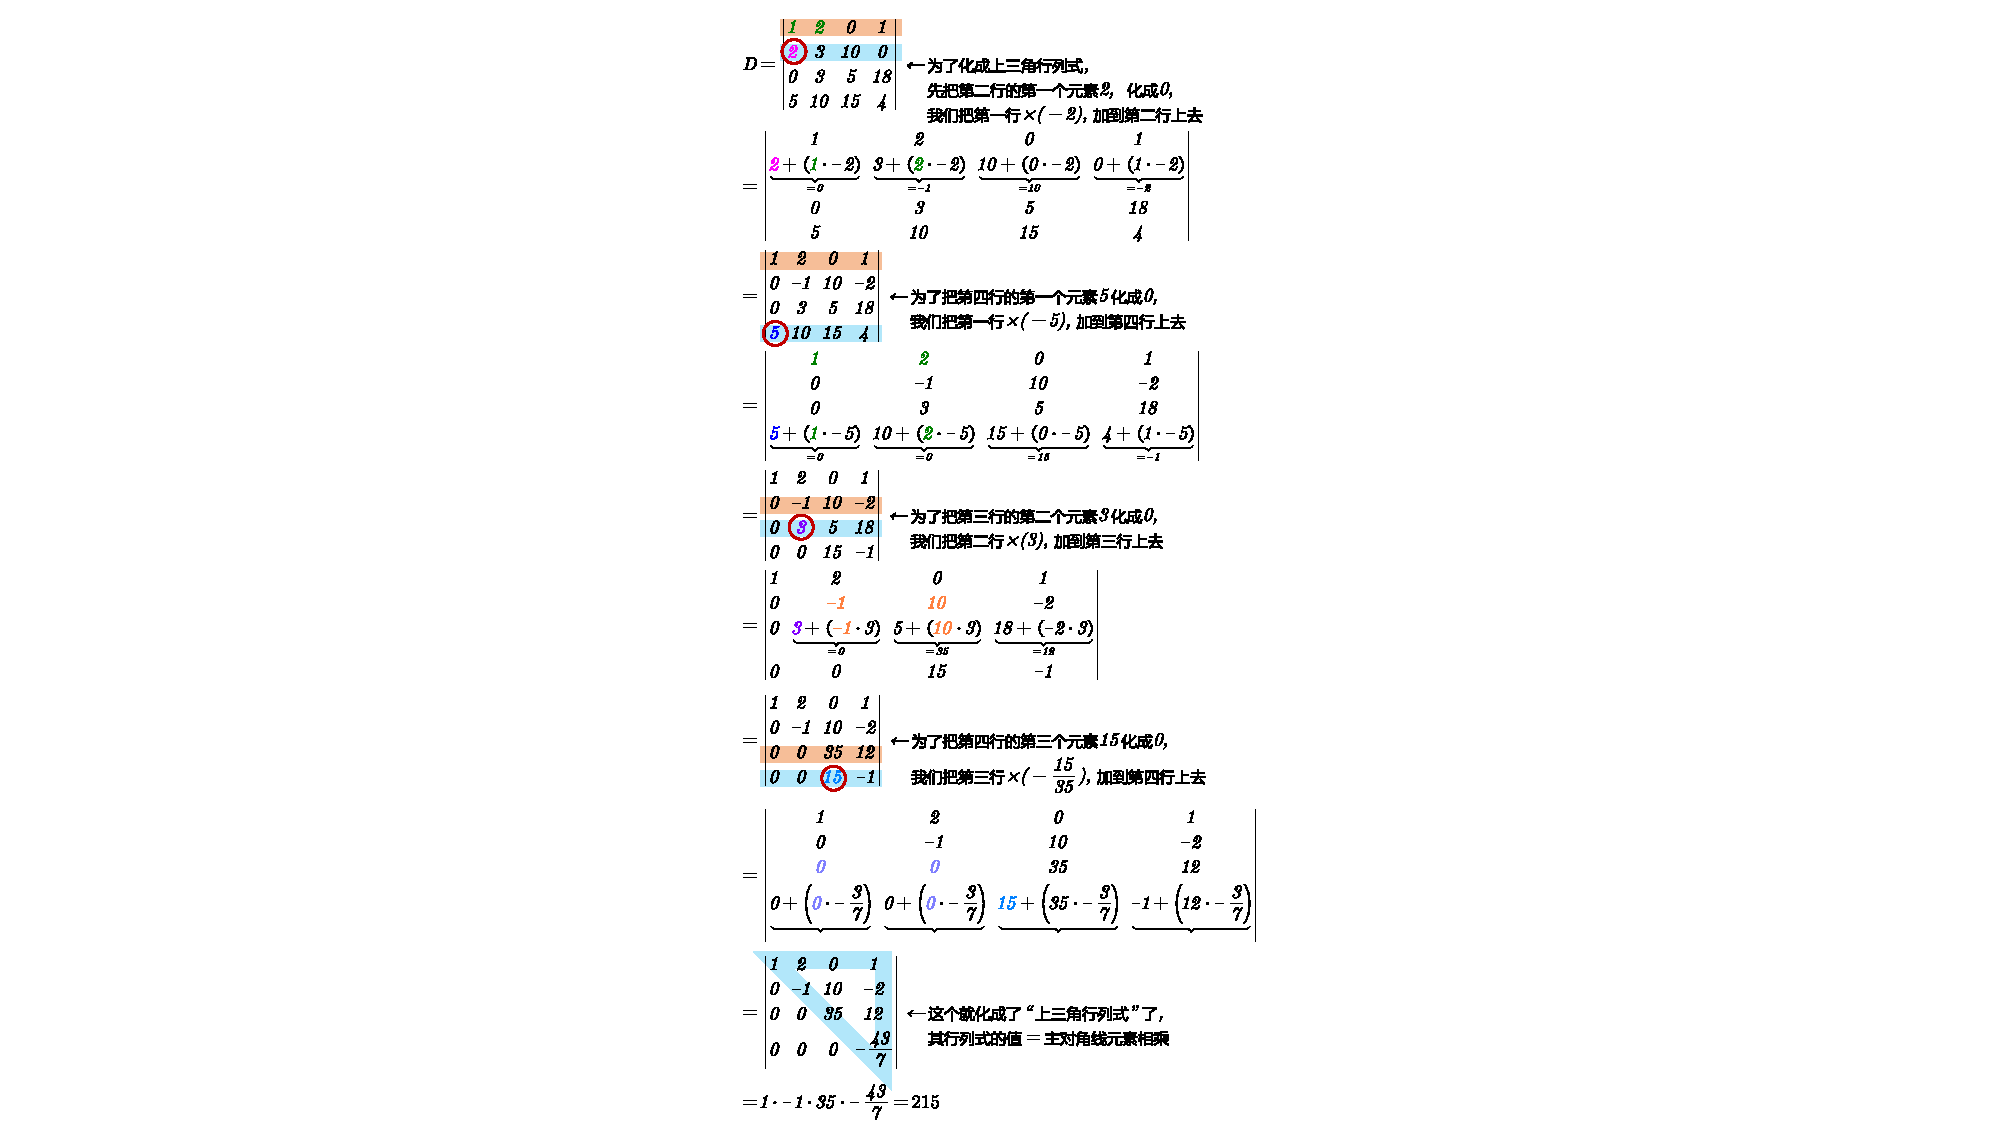
\includegraphics[width=0.75\textwidth]{img/0010.pdf}\\
	
	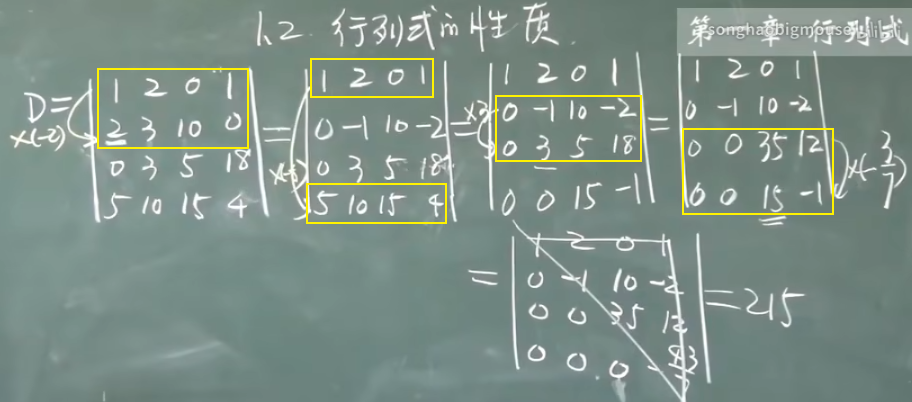
\includegraphics[width=0.75\textwidth]{img/0011.png}\\
	
	总结:\\
	1.先处理第1列, 再处理第2列, 再处理第3列. \\
	2.第1列处理完后, 第1行就不再参与运算. \\
	
	
	
	
	
	

	\hrule

	
	\subsection{如果某一行的首元素是1, 就把该行移到第一行上去} 
	
	比如: \\
	$
	\left| \begin{matrix}
		8&		&		\\
		1&		...&		\\
		3&		&		\\
	\end{matrix} \right|
	$\\
	
	第二行的首元素是1, 就把这第二行, 移到第1行上去. 变成: \\	
		$
	\left| \begin{matrix}
		1&		...&		\\
		8&		&		\\
		3&		&		\\
	\end{matrix} \right|
	$\\
	
	这样, 能更方便的用第一行元素乘以某个数, 来消去下面行上的数字, 以变成0. 化成``上三角行列式". \\
	注意: 在交换两行时, 行列式的值要变号. \\


\hrule

		
	\section{行列式按行(列)展开}
	
		\subsection{余子式 minor :  $M_{ij}$}
		
		你选定某个元素x, 把它所在的行去掉, 所在的列去掉, 将剩下的元素按原位置排好, 这个新的行列式, 就是x的``余子式". \\
		
		比如: \\
		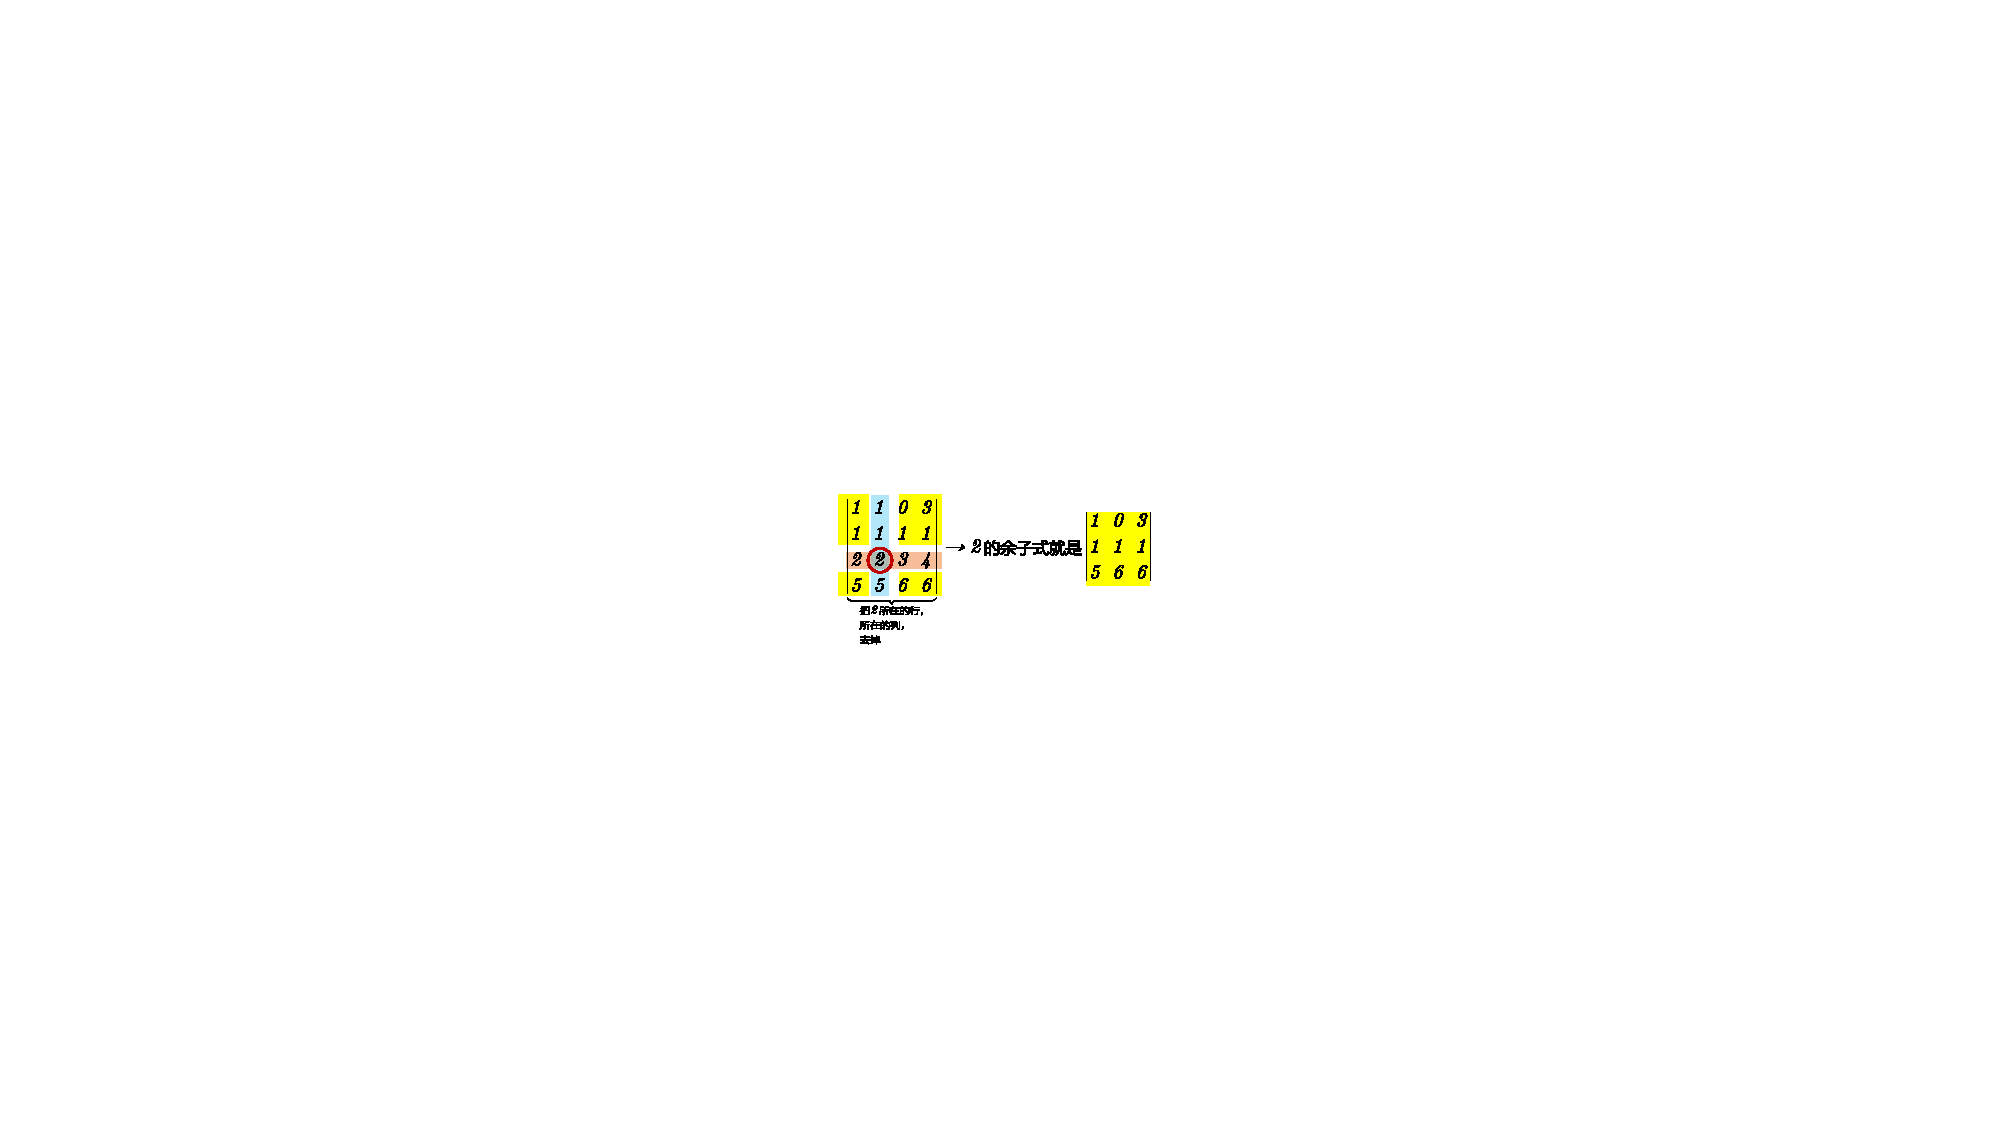
\includegraphics[width=0.4\textwidth]{img/0012.pdf}\\
		
		某个元素的余子式, 用 $M_{ij}$表示. 如, 上例中的2, 在 i=第3行, j=第2列, 所以它的``余子式"就是: \\
		$
		M_{32}=\left| \begin{matrix}
			1&		0&		3\\
			1&		1&		1\\
			5&		6&		6\\
		\end{matrix} \right|
		$ \\
		

		\hrule

		
	\subsection{代数余子式 Algebraic cofactor : $	A_{ij}=\left( -1 \right) ^{i+j}M_{ij}$}
		
	在余子式的前面, 加一个负号, 即 $\left( -1 \right) ^{i+j}	$, 就是``代数余子式". \\
	 某个元素x的``代数余子式", 用符号 $A_{ij}$ 来表示. i是x的行号, j是x的列号.\\
	 
	比如上例的``余子式"是: \\
		$
	M_{32}=\left| \begin{matrix}
		1&		0&		3\\
		1&		1&		1\\
		5&		6&		6\\
	\end{matrix} \right|
	$ \\
	
	那么其``代数余子式"就是: \\
	$
	A_{32}=\left( -1 \right) ^{3+2}\left| \begin{matrix}
		1&		0&		3\\
		1&		1&		1\\
		5&		6&		6\\
	\end{matrix} \right|
	$ \\
	
	

	\hrule


\subsection{按某一行(列)展开的展开公式: \\ $|A|=\sum_{i=1}^n{a_{ij}A_{ij}\ \left( j=1,2,...,n \right)}=\sum_{j=1}^n{a_{ij}A_{ij}\ \left( i=1,2,...,n \right)}$	}

有定理: \textbf{行列式的值等于: 随便选一行, 把这行上所有的元素, 各自乘以它们的``代数余子式", 再求和, 所得到的结果, 就是这个行列式的值了.} 
\begin{align*}
	\boxed{
		D=\underset{\text{某一行的元素}}{\underbrace{a_{i1}}}\cdot \underset{\text{该元素的}“\text{代数余子式}”}{\underbrace{A_{i1}}}+a_{i2}\cdot A_{i2}+...+a_{in}\cdot A_{in}		
	}
\end{align*}
	
	用列来做, 也是一样. \\
	$
	D=\underset{\text{某一列的元素}}{\underbrace{a_{1j}}}\cdot \underset{\text{该元素的}“\text{代数余子式}”}{\underbrace{A_{1j}}}+a_{2j}\cdot A_{2j}+...+a_{nj}\cdot A_{nj}
	$	\\
	
	\begin{myEnvSample}
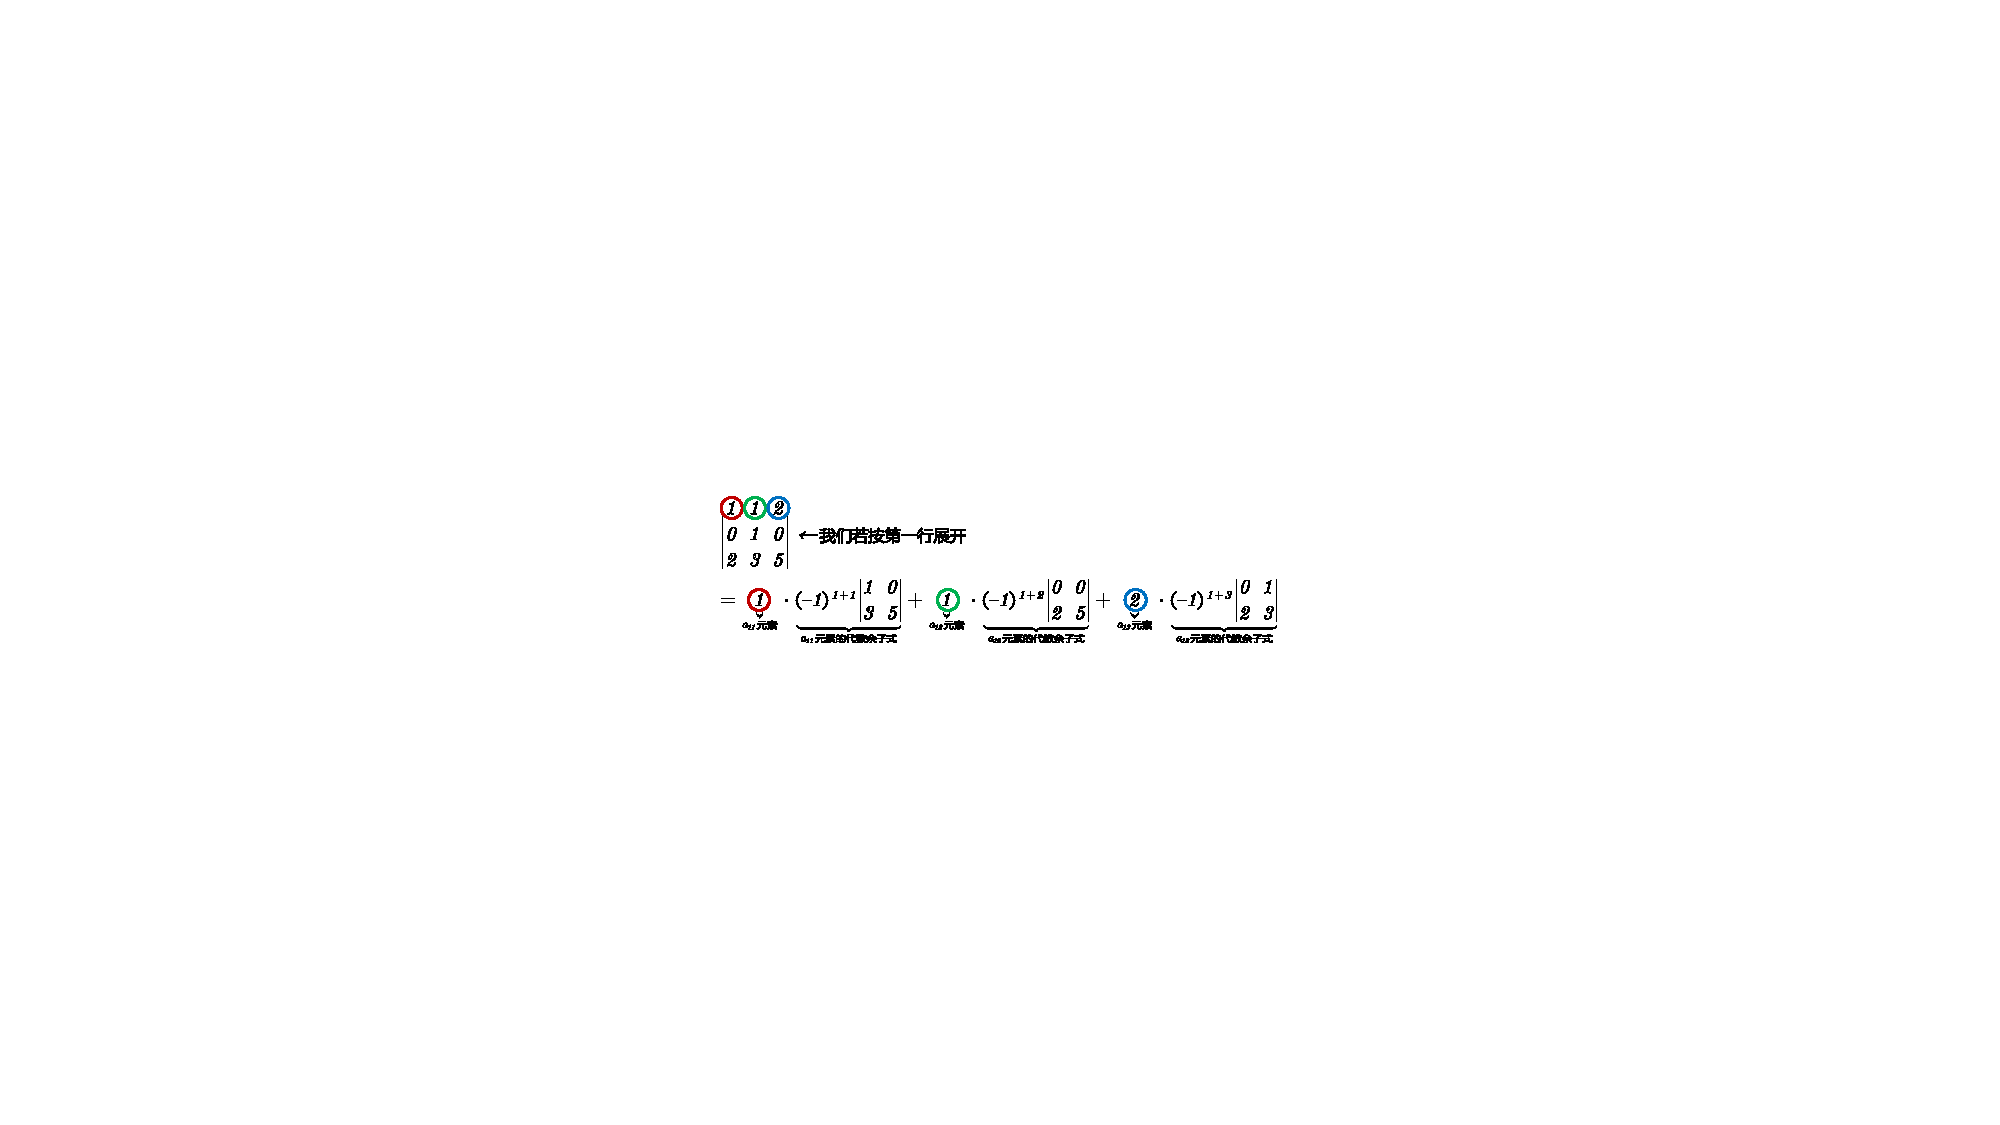
\includegraphics[width=0.8\textwidth]{img/0013.pdf}
	\end{myEnvSample}
	
	从上例, 你就能发现, ``行列式"按行或列展开后, 它的每一个元素的代数余子式, 都``降阶"了. 即 原行列式是3阶的, 现在展开后, 你只要计算 2阶的行列式(即代数余子式)了. 大大减轻了我们的计算负担. \\
	
	其实, 上面的这个例子, 我们按第二行展开更方便, 因为它有0元素存在啊, 0元素和其代数余子式相乘, 就是0. 根本就不需要我们去计算了. 所以, \textbf{我们要选0元素最多的那一行来展开} : \\
	\begin{myEnvSample}
	\begin{align*}
	& \left| \begin{matrix}
		1&		1&		2\\
		0&		1&		0\\
		2&		3&		5\\
	\end{matrix} \right|\ ←\text{要选0元素最多的那一行来展开,本例即第二行}\\
	& =0+\underset{a_{22}\text{元素}}{1}\cdot \underset{a_{22}\text{元素的代数余子式}}{\underbrace{\left( -1 \right) ^{2+2}\left| \begin{matrix}
				1&		2\\
				2&		5\\
			\end{matrix} \right|}}+0
\end{align*}
	\end{myEnvSample}
	

	

	\hrule

	
	\section{异乘变零定理}
	
	即: \textbf{某行上的元素, 与另一行(即别人的行)上对应元素的"代数余子式"相乘, 将所有的乘积值, 再全加起来, 其和 =0.} \\
	
	如: (1) \\
	$
	\begin{matrix}
		\left| \begin{matrix}
			1&		1&		2&		3\\
			\hline
			0&		0&		8&		9\\
			2&		5&		5&		4\\
			9&		9&		9&		10\\
			\hline
		\end{matrix} \right|\\
	\end{matrix}
	$\\
	
	用第4行, 与第1行元素的``代数余子式"相乘, 再把相乘后的值, 全加起来, 则:\\
	$ D= a_{41}A_{11} + a_{42}A_{12} + a_{43}A_{13} + a_{44}A_{14} = 0$ \\
	
	``异乘变零定理"的证明过程: \\	
	比如这个行列式(2): \\
	
	$
	\begin{matrix}
		\left| \begin{matrix}
			9&		9&		9&		10\\
			\hline
			0&		0&		8&		9\\
			2&		5&		5&		4\\
			9&		9&		9&		10\\
			\hline
		\end{matrix} \right|\\
	\end{matrix}
	$ \\
	
	其中, 1,4行相同. 即两行相同, 则该行列式的值=0. \\
	若用第1行展开, 你会发现, 展开的式子, 与上面的行列式(1), 完全相同. 既然这边的(2)是0, 那么上面的(1)也是0了. 证毕. 
	
	
	
	
	
	
~\\
\hrule
~\\
	
	\section{拉普拉斯定理}
	
	\subsection{k阶子式}
	
	就是从一个n阶行列式中, 随便取k行, 取k列, 组成的新的行列式, 就是k阶子式. \\
	比如:\\
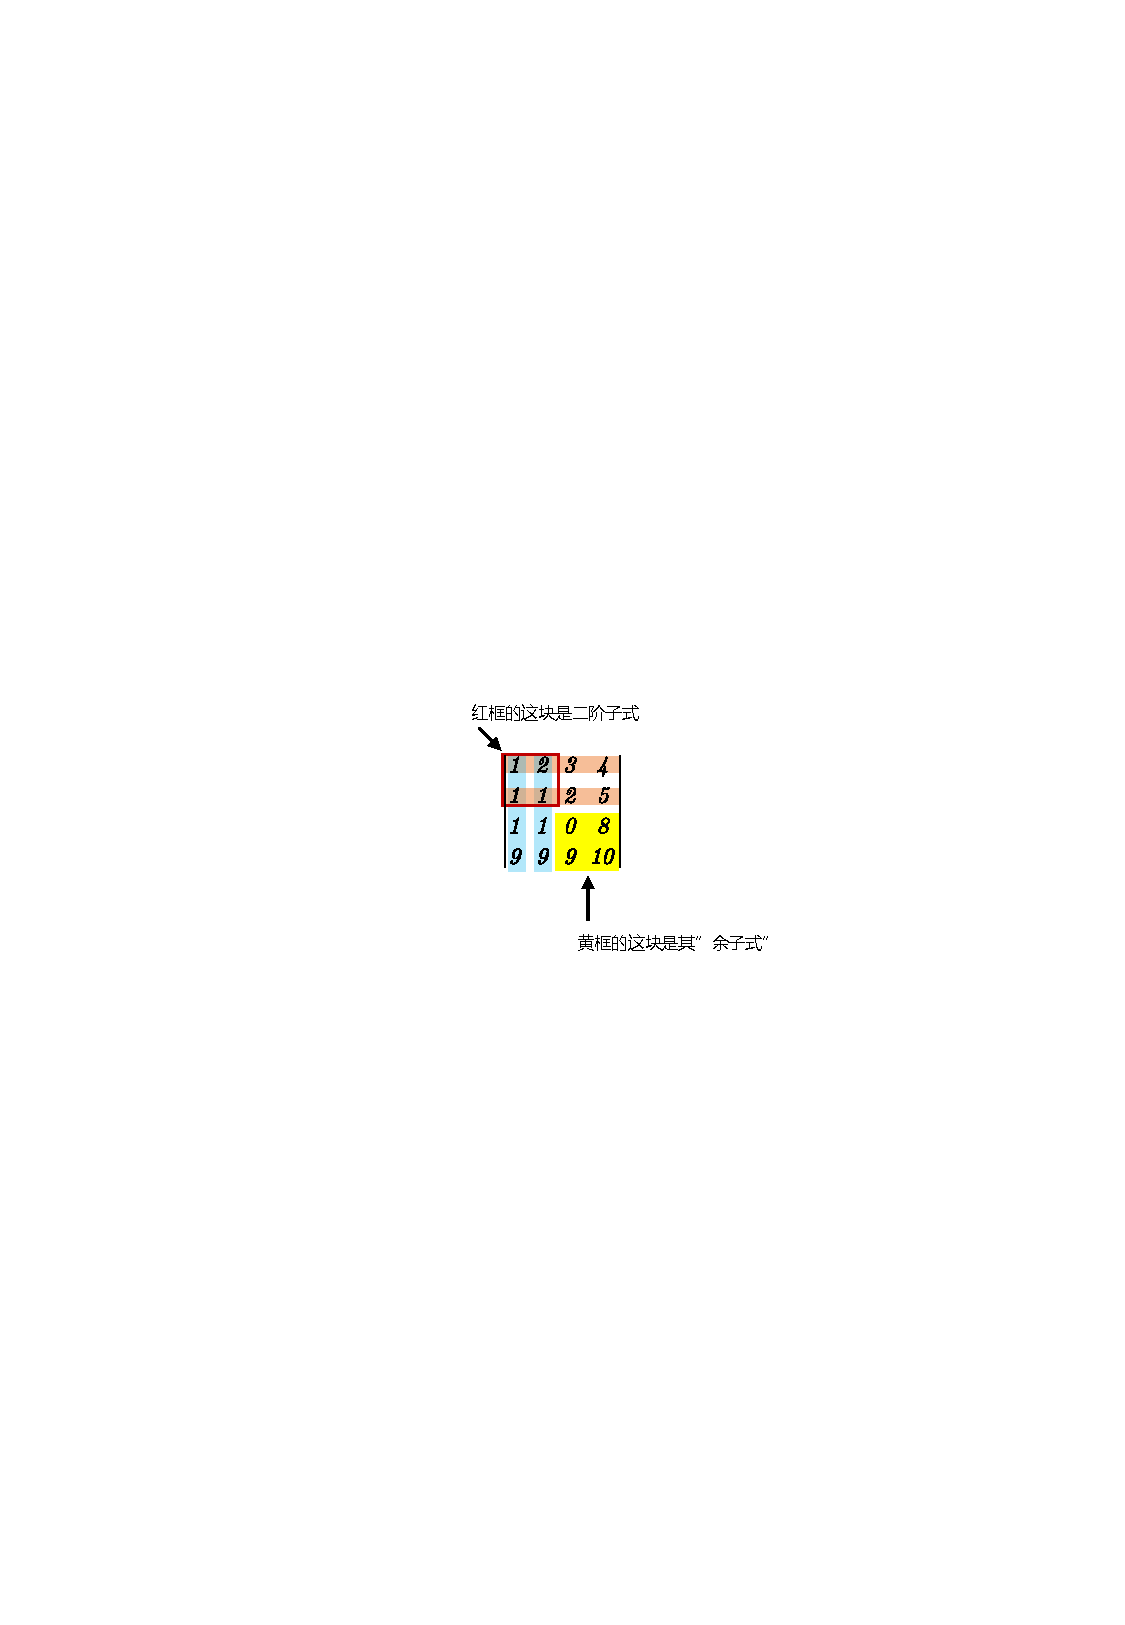
\includegraphics[width=0.35\textwidth]{img/0014.pdf} \\

我们取出它一个2阶子式 (即2*2区域的子集). 比如, 就取第1,2行,和第1,2列 交叉点, 所组成的子式, 即:
$
\left| \begin{matrix}
	1&		2\\
	1&		1\\
\end{matrix} \right|
$
	这个就是一个``二阶子式". \\
	
	那么这个二阶子式的``余子式", 就是:
$
\left| \begin{matrix}
	0&		8\\
	9&		10\\
\end{matrix} \right|
$	\\




这个二阶子式的``代数余子式", 就是: \\
$
\left( -1 \right) ^{\overset{\text{行1,行}2}{\overbrace{\left( 1+2 \right) }}\overset{\text{列1,列}2}{\overbrace{\left( 1+2 \right) }}}\left| \begin{matrix}
	0&		8\\
	9&		10\\
\end{matrix} \right|
$ \\

	注意: 上面 -1 的指数, 两个括号的意思是:
	\begin{align*}
		\left| \begin{matrix}
			0&		8\\
			9&		10\\
		\end{matrix} \right|
	\end{align*}
	

	~\\
	\hrule
	~\\

	\subsection{拉普拉斯展开定理}
	
	\textbf{拉普拉斯展开定理 Laplace expansion : 在n阶行列式中, 任意取定k行(而不仅仅是只取一行展开), 由k行元素组成的所有``k阶子式"与``代数余子式"的乘积之和, 就等于该行列式的值.} \\
	
	\begin{myEnvSample}
	如: 下面这个5阶行列式 \\
	
	$
		\left| \begin{matrix}
			1&		2&		0&		0&		0\\
			\hline
			3&		4&		0&		0&		0\\
			\hline
			1&		2&		3&		4&		5\\
			1&		1&		1&		1&		1\\
			6&		6&		8&		3&		1\\
		\end{matrix} \right|
	$\\
	
	我们任取k=2行, 比如就取 第1, 2 行. 它的k阶子式, 就是二阶子式. 那么因为这个行列式有5列, 在其中取2列, 就有$C_{5}^{2}=10$种取法. 即有10个二阶子式存在. \\
	即, \textbf{这个5阶行列式的值 D=  (第1个二阶子式的行列式值×其代数余子式) + (第2个二阶子式的行列式值×其代数余子式) + ... + (第10个二阶子式的行列式值×其代数余子式)} \\
	
	如果我们取到的是``列上都是0元素"的那些列的话, 那么这个二阶子式的行列式的值就是0了. 其``二阶子式"与``代数余子式"的乘积之和, 当然也是0了. \\
	所以, 在全部10个二阶子式中,  唯一行列式值不为零的二阶子式, 就是取第1和第2列. 它的``二阶子式"值×其``代数余子式" = $
	\underset{\text{二阶子式}}{\underbrace{\left| \begin{matrix}
				1&		2\\
				3&		4\\
			\end{matrix} \right|}}\cdot \underset{\text{代数余子式}}{\underbrace{\left( -1 \right) ^{\left( 1+2 \right) +\left( 1+2 \right)}\left| \begin{matrix}
				3&		4&		5\\
				1&		1&		1\\
				8&		3&		1\\
			\end{matrix} \right|}}
	$ \\
	
	即, 本例的这个5阶行列式的值 = $
	\underset{\text{二阶子式}}{\underbrace{\left| \begin{matrix}
				1&		2\\
				3&		4\\
			\end{matrix} \right|}}\cdot \underset{\text{代数余子式}}{\underbrace{\left( -1 \right) ^{\left( 1+2 \right) +\left( 1+2 \right)}\left| \begin{matrix}
				3&		4&		5\\
				1&		1&		1\\
				8&		3&		1\\
			\end{matrix} \right|}} + 0 + 0 + ...
	$ \\
	\end{myEnvSample}	
	
	

	\hrule

	\section{行列式相乘}
	
	\subsection{两个``同阶"行列式 相乘}
	
	两个同阶行列式, 相乘, 方法是:  \textbf{前行×后列} \\	
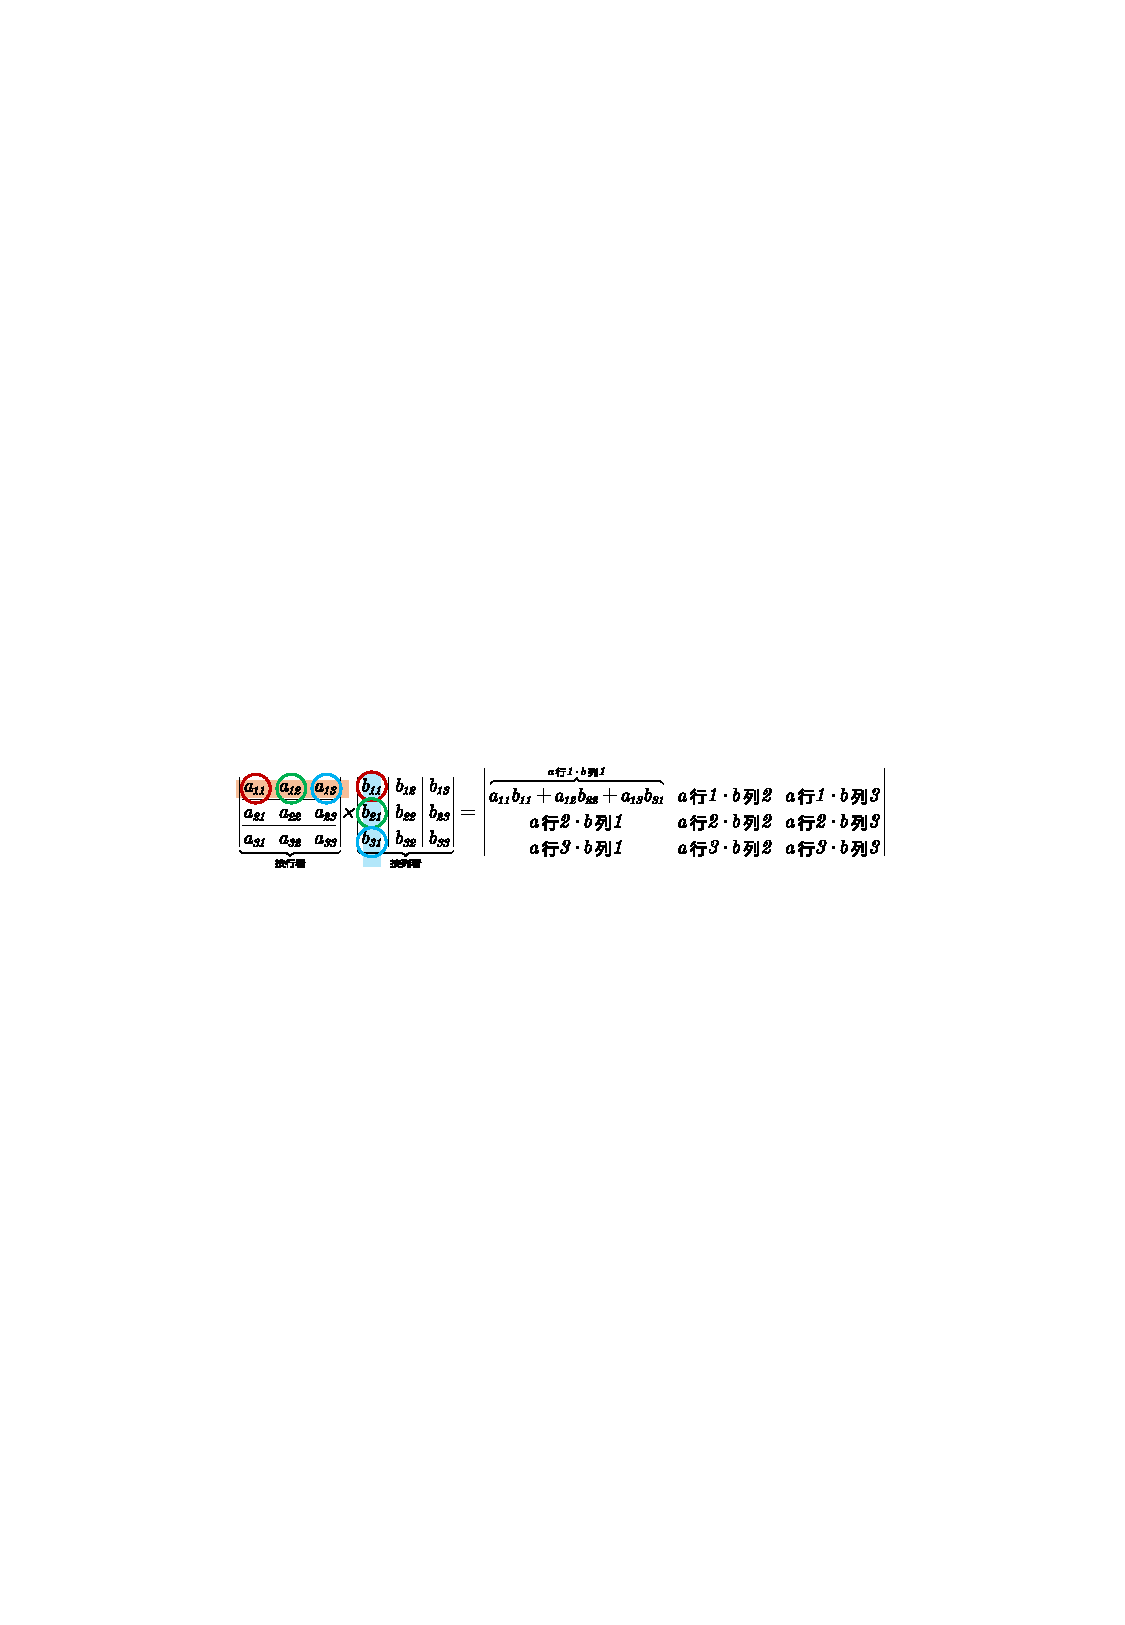
\includegraphics[width=0.9\textwidth]{img/0015.pdf}


~\\
\hrule
~\\


	
	\subsection{两个``不同阶"行列式 相乘}
	
那就只能先算出各自行列式的值, 再来相乘了.
	
	
	
	
	\begin{myEnvSample}

	\end{myEnvSample}
	
	
	
	
	--------------------------------
	
	\section{n阶行列式}
	
	
	\section{行列式的性质}
	
	\subsection{性质1: 行列互换, 其值不变. 即$|A|=\left| A^T \right|$}
	
	\subsection{性质2: 某行(列)元素全为零, 则行列式为零}
	
	\subsection{性质3: 两行(列)元素相等, 或对应成比例, 则行列式为零}
	
	\subsection{性质4: 某行(列)元素均是两个元素之和, 则可拆成两个行列式之和}
	
	\subsection{性质5: 两行(列)互换,行列式的值反号}
	
	\subsection{性质6: 某行(列)元素有公因子$k\left( k\ne 0 \right) $, 则k可提到行列式外面去 }
	
	\subsection{性质7: 某行(列)的b, 倍加到另一行(列)上去, 行列式的值不变 }
	
	
	\section{行列式的展开定理}
	
	\subsection{余子式 $M_{ij}$}
	
	\subsection{代数余子式 $	A_{ij}=\left( -1 \right) ^{i+j}M_{ij}$}
	
	\subsection{按某一行(列)展开的展开公式: \\ $|A|=\sum_{i=1}^n{a_{ij}A_{ij}\ \left( j=1,2,...,n \right)}=\sum_{j=1}^n{a_{ij}A_{ij}\ \left( i=1,2,...,n \right)}$	}
	
	
	
	\section{具体型行列式的计算: $a_{ij}$ 已给出}
	
	\subsection{化为``12+1"型行列式}
	
		\subsubsection{主对角线行列式}
		
		\subsubsection{副对角线行列式}
		
		\subsubsection{拉普拉斯展开式}
		
		\subsubsection{范德蒙德行列式}
	
	\subsection{加边法}
	
	\subsection{递推法 (高阶 → 低阶)}
	
		\subsubsection{建立递推公式,即建立$D_n$ 与 $D_{n-1}$ 的关系}
		
		\subsubsection{$D_n$ 与 $D_{n-1}$ 要有完全相同的元素分布规律, 只是$D_{n-1}$比$D_n$低了一阶 }
	
	
	\subsection{数学归纳 (低阶 → 高阶)}
	
		\subsubsection{第一数学归纳法}
		
		\subsubsection{第二数学归纳法}
	
	
	\section{抽象型行列式的计算: $a_{ij}$ 未给出	}
	
		\subsection{用行列式性质}
		
		\subsection{用矩阵知识}
		
			\subsubsection{设 C=AB, A,B为同阶方阵, 则 $|C|=|AB|=|A||B|$}
			
			\subsubsection{设 C=A+B, A,B为同阶方阵, 则 $|C|=|A+B|$,作恒等变形,转化为矩阵乘积的行列式 }
			
			\subsubsection{设A 为n阶方阵, 则 $|A^*|=|A|^{n-1},\ |(A^*)^*|=\left| \left| A \right|^{n-2}A \right|=\left| A \right|^{\left( n-1 \right) ^2}	$}
		
		\subsection{用相似理论}
		
			\subsubsection{$\left| A \right|=\prod_{i=1}^n{\lambda _i}$}
			
			\subsubsection{若A相似于B, 则 |A|=|B|}
	
	
	
\end{document}